% --------------------------------------------------------------------

\chapter[Cosmology]{Keeping It Even: Accurate Cosmological Measurements on the Largest Scales}
\def\chpname{cosmo}\label{chp:\chpname}

Chapter editors:
\credit{egawiser},
% {\it Peter Kurczynski},
% \credit{drphilmarshall},
% \credit{ohadshemmer},
% \credit{tanguita},
% \credit{jmeyers314},
\credit{MichelleLochner}.
% \credit{jhrlsst},
% \credit{rbiswas4}
% {\it and others to follow}

% --------------------------------------------------------------------

\section{Introduction}
\label{sec:\chpname:intro}

% Introduce, with a very broad brush, this chapter's science projects,
% and why it makes sense for them to be considered together.

Cosmology is one of the key science themes for which LSST was
designed. Our goal is to measure cosmological parameters, such as the
equation of state of dark energy, or departures from General
Relativity, with sufficient accuracy to distinguish one model from
another, and hence drive our theoretical understanding of how the
universe works, as a whole. To do this will necessarily involve a
variety of different measurements, that can act as cross-checks of
each other, and break parameter degeneracies in any single one.

The  Dark Energy Science Collaboration (DESC) has identified five
different cosmological probes enabled by the LSST: weak lensing (WL),
large scale structure (LSS), type Ia supernovae (SN), strong lensing
(SL), and clusters of galaxies (CL). In all cases, the primary concern
is residual systematic error: the shapes and photometric redshifts of
galaxies, and the properties of supernova and lensed quasar light
curves, will all need to be measured with extraordinary accuracy in order for LSST's high statistical power to be properly harnessed. This accuracy will come from the abundance and heterogeneity of the individual measurements made, and the degree to which they can be modeled and understood. This latter point implies a need for uniformity in the survey, which enables powerful simplifying assumptions to be made when calibrating on the largest, cosmologically most important scales. The need for heterogeneity also implies  uniformity, in the sense that the nuisance parameters that describe the systematic effects need to be sampled over as wide a range as possible (examples include the need to sample a wide range of roll angles to minimize shape error, and observing conditions to understand photometric errors due to the changing atmosphere).

In this chapter we look at some of the key measurements planned by the
Dark Energy Science Collaboration, and how they depend on the
Observing Strategy.


%---------------------------------------------------------------------

% ====================================================================
%+
% SECTION NAME:
%    photoz.tex
%
% CHAPTER:
%    cosmology.tex
%
% ELEVATOR PITCH:
%    Photometric redshifts are an intermediate data product that comprises
%    a key input for many investigations of galaxies and cosmology.  They
%    represent "static science", but we need them to have high quality after
%    the first year and at each "data release" thereafter.
%
% COMMENTS:
%    Updated Wed May 18 by MLG.
%    Minor updates to figures and captions, Sep 14 by MLG.
%    Updated figures and parts of the text, and responded to
%      comments from David Kirkby (issue #633) May 11 2017, MLG.
%
% BUGS:
%
%
% AUTHORS:
%   Melissa Graham, Sam Schmidt, Andy Connolly, Zeljko Ivezic
%-
% ====================================================================
\clearpage
\section{Photometric Redshifts}
\def\secname{photoz}\label{sec:\secname}

\credit{MelissaGraham},
\credit{SamSchmidt},
\credit{connolly},
\credit{ivezic}

\subsection{Introduction}

Photometric redshifts are an essential part of
every cosmology probe within LSST.  The principal concern for LSST
photo-$z$ performance is to meet the stringent requirements on redshift
uncertainty, bias, and catastrophic outlier rate as laid out in the
Science Requirements document. Photo-$z$'s are dependent on precise
measurements of galaxy colors, thus cadence and depth variations must be
examined as a function of all six LSST filter bandpasses.  Overall image
depth and signal-to-noise is our primary concern. For studies of Large
Scale Structure, Weak Lensing, Clusters, and Supernova host galaxies,
survey uniformity is desired for the full depth survey, while the
temporal details of how we reach full depth are not as important as
uniformity both as a function of sky position and observing conditions.
However, as we desire science-grade photometric redshifts after one year
of operations, two years, and so forth, the cadence must meet some basic
requirements for the six-band system at least on the timescales of the
yearly data releases.

\textbf{Specifications.} The Science Requirements Document (SRD; \citealt{LPM-17}) defines
the minimum statistical specifications for photometric redshifts for an
$i<25$, magnitude-limited sample of $4\times10^9$ galaxies from
$0.3<z<3.0$ as: (1) the root-mean-square of the error in photo-$z$
must be $\sigma < 0.02$; (2) the fraction of outliers must be $<10\%$;
and (3) the average bias must be $<0.003$.
The details for how these statistics are calculated are discussed in the Metrics section below.
With this in mind, we are developing software to show that our photo-$z$ algorithms
can meet specifications for LSST baseline parameters and to simulate the
impact of deviations from the 10-year baseline plan on photo-$z$
statistics.

\textbf{Planned Experiments.} This software is designed to allow the
user to modify LSST baseline parameters, simulate a set of test galaxy
observations (i.e., magnitudes with errors appropriate for the given
LSST parameters) from a training catalog with ``true" magnitudes and
redshifts and a realistic intrinsic dispersion in color, magnitude, and
redshift, run a photometric redshift algorithm on the test galaxies
(i.e., matching in color-space to the training catalog), and output
statistics for analysis. Modifiable LSST input parameters will include:
the limiting magnitude applied to the galaxy catalogs (e.g., $i<25$);
the number of visits per filter; the number of years of LSST
observations that have passed (this can be a fraction of a year);
systematic offsets to the magnitudes in each filter (default $=0$); and
coefficients for the magnitude uncertainties in each filter (default
$=1$).  Output for user analysis will include catalogs of $z_{\rm phot}$
and the metrics for photo-$z$
in any desired redshift range. For example, we will be able to vary the
total number of $u$-band visits and examine how this affects the
fraction of outliers at 1, 5, and 10-years of the survey. In this
software, parameters of the photo-$z$ algorithm itself will also be
modifiable, allowing us to test options in the algorithms against
various LSST observing strategies.

\textbf{Currently implemented photo-$z$ algorithm.} We draw $N_{\rm
test}$ ``test" and $N_{\rm train}$ ``training" galaxies from a catalog of
simulated galaxies, ensuring no overlap. We determine their
magnitude uncertainties as appropriate for the LSST parameters, randomly
scatter their magnitudes to induce an observational error, and calculate
the associated colors and color errors. 
We calculate the Mahalanobis distance \citep{Mahalanobis1936} in color space
between each test galaxy and the 10\% of training set galaxies closest matched
in apparent $i$-band magnitude (i.e., thereby applying a crude prior on magnitude),
and then use it to identify a color-matched subset of
training galaxies using a threshold defined by the $\chi^2$ percentage point function at 68\%.
We draw a random training galaxy from this subset and use its redshift as the
photo-$z$ for that test galaxy. We then calculate our statistical
metrics on the photometric redshifts for the test sample, using each
test galaxy's original catalog redshift as the ``true'' redshift.
Our adopted method is not necessarily the ``best" way to calculate photometric redshifts,
but due to its relatively direct relation between the photometric errors
and the uncertainty in the estimated photo-$z$, it is especially appropriate analyzing the impact of changes
to the LSST observing strategy.
Also, this process is open to substituting alternate photometric redshift
algorithms, a variety of galaxy catalogs, and/or adding different priors.
Note that for this experiment, we always assume that the
training set galaxies have photometric errors equivalent to that of the
full-depth (i.e., 10-year) LSST catalog. 

\subsection{Metrics}

The primary metrics we will use to evaluate LSST
observing strategies with respect to the SRD photo-z specifications are the
robust standard deviation, the robus bias, and the fraction of outliers. For all test
galaxies we calculate $\Delta z = (z_{\rm true} - z_{\rm phot}) /
(1+z_{\rm phot})$, and identify galaxies in the interquartile range (IQR) of $\Delta z$.
The robust standard deviation is calculated by dividing the full-width of the IQR by 1.349 (i.e., assuming a Gaussian distribution, which we find to be appropriate).
The robust bias is the mean value of $\Delta z$ for IQR galaxies.
Outlier galaxies are identified as those with $\Delta z$ exceeding the larger of 0.06 or 3$\sigma$, 
where $\sigma$ is the robust standard deviation for all galaxies with $0.3 \leq z_{\rm phot} \leq 3.0$.
The IQR is used to exclude outliers from influencing these statistics; in other words, the robust
standard deviation and bias are for a subset of ``good" photo-$z$'s.

\subsection{Initial Results}

To demonstrate this software with a
preliminary analysis, we apply the currently implemented photo-$z$
algorithm to a galaxy catalog based on the Millennium simulation \citep{2005Natur.435..629S},
which uses the galaxy formation models of \citep{2014MNRAS.439..264G}
and was constructed using the lightcone techniques described by \cite{2013MNRAS.429..556M}.
We use $N_{\rm train}=1000000$ and $N_{\rm test}=50000$ galaxies, and apply the 
condition of $i<25$ after scattering based on their magnitude errors in order
to generate a sample for which the LSST SRD specifications apply.
For this demonstration we show how the photo-$z$ metrics evolve with respect to
two of the basic LSST parameters: the year of the survey, and the number
of $u$-band visits. When we simulate results in a given year of LSST, we
assume uniform progression in all filters (i.e., the total number of
visits per filter, \texttt{[56, 80, 184, 184, 160, 160]} in
\texttt{[u,g,r,i,z,y]}, is distributed evenly over all years). When we
simulate the LSST 10-year results for a given number of $u$-band visits,
the visits removed/added to $u$-band are added/subtracted evenly to/from
the other five filters. The results of these tests are presented in
Figure~\ref{fig:redshifts} and~\ref{fig:metrics}. For example, in this
demonstration we can see how the photo-$z$ results will improve
over time, and how the fraction of outliers at low $z_{\rm phot}$ actually increases
for the first half of the survey as the standard deviation improves.
We can also see that a lack of $u$-band data induces more scatter 
in the photo-$z$ results at $z<0.5$ and $z>2.0$, but that allotting 
more than 56 visits to $u$-band does not necessarily improve the results,
since this comes at the expense of visits in the other filters.

\begin{figure}[h]
\begin{center}
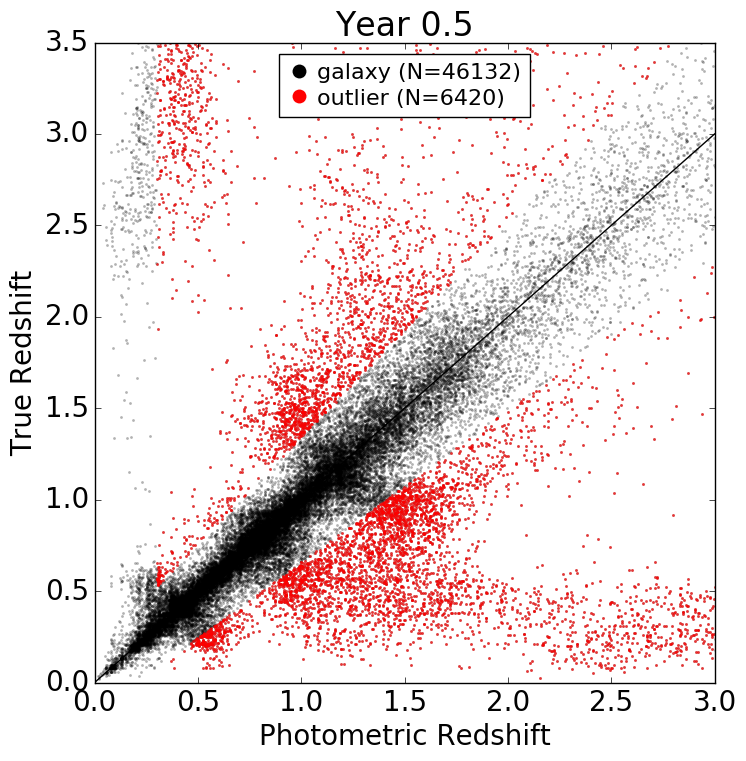
\includegraphics[width=5cm]{figs/photoz/pztz_nyears_p5.png}
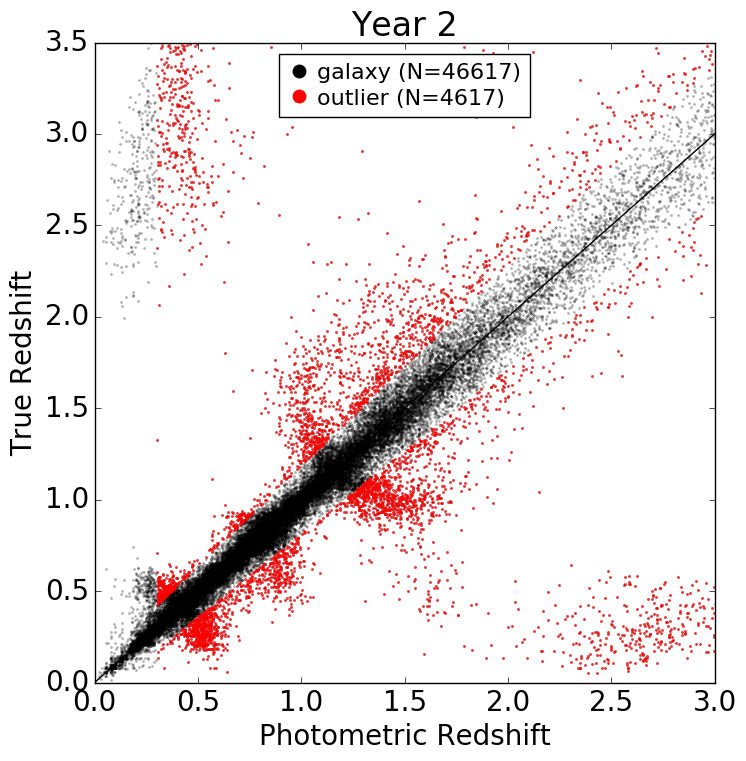
\includegraphics[width=5cm]{figs/photoz/pztz_nyears_2.png}
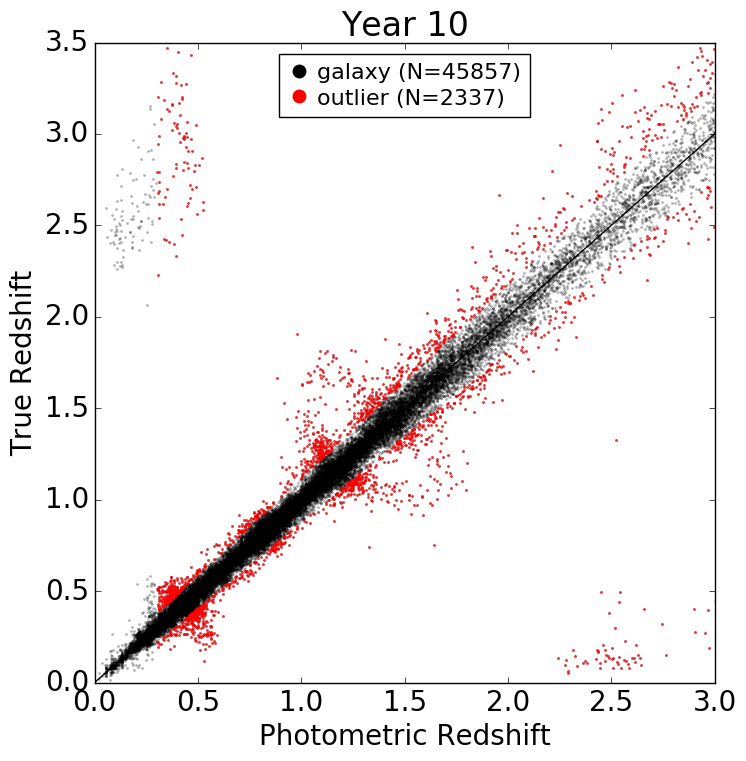
\includegraphics[width=5cm]{figs/photoz/pztz_nyears_10.png}
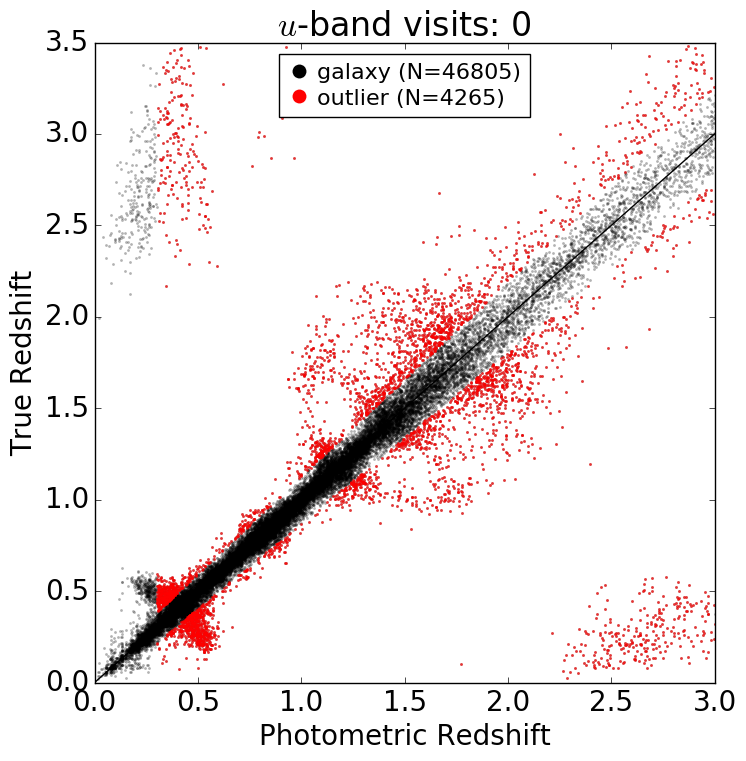
\includegraphics[width=5cm]{figs/photoz/pztz_uvisits_0.png}
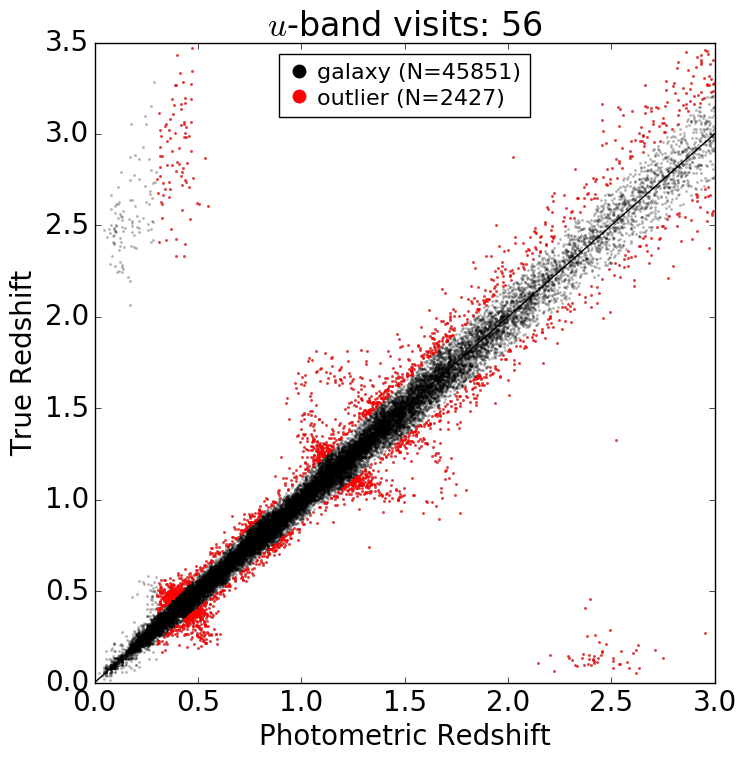
\includegraphics[width=5cm]{figs/photoz/pztz_uvisits_56.png}
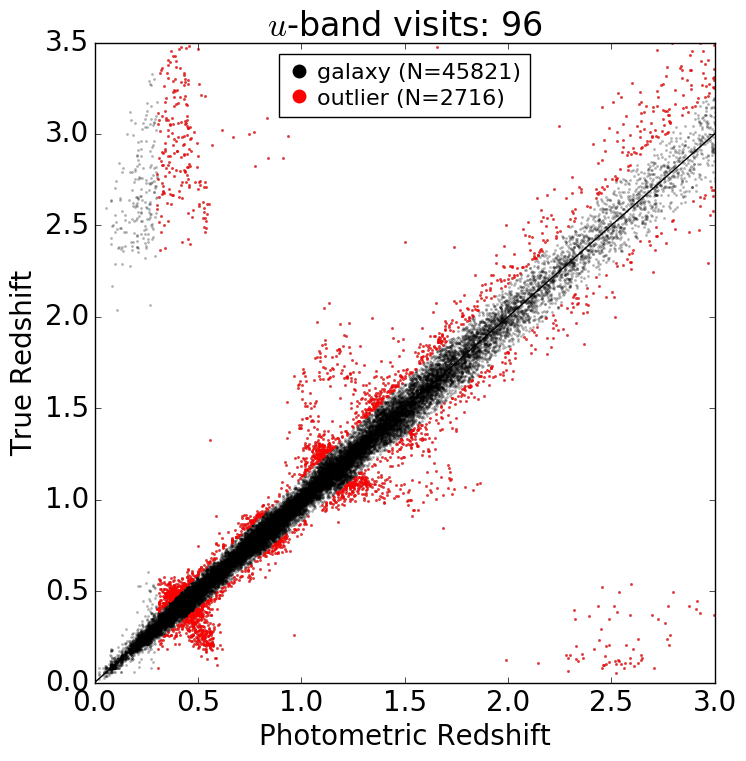
\includegraphics[width=5cm]{figs/photoz/pztz_uvisits_96.png}
\caption{Photometric vs. true (i.e., catalog) redshifts. Across the top row we show results from
0.5, 2.0 and 10.0 years of the LSST survey, and across the bottom row we show results for $0$,
$56$ (baseline), and $96$ $u$-band visits. 
\label{fig:redshifts}}
\end{center}
\end{figure}

\begin{figure}[h]
\begin{center}
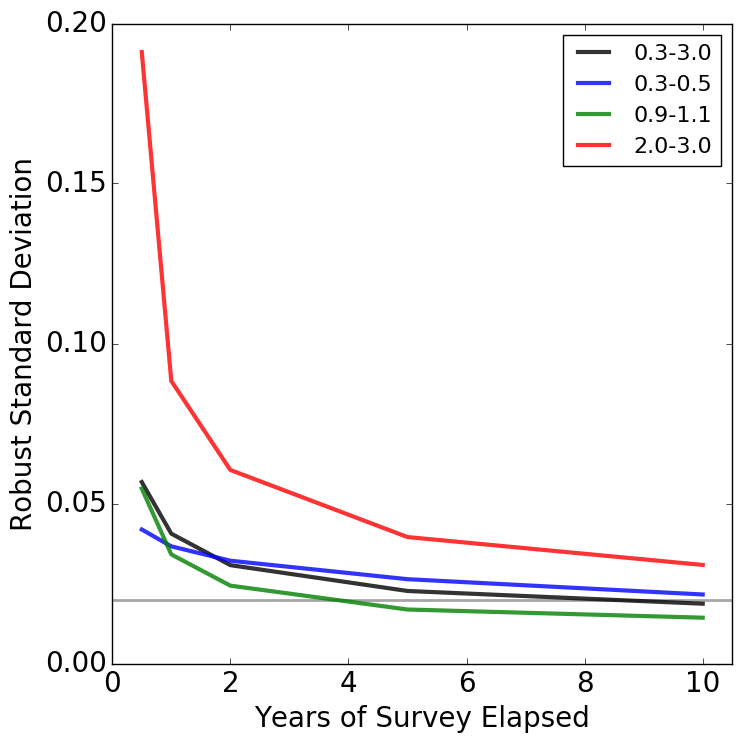
\includegraphics[width=5cm]{figs/photoz/pstat_nyears_IQRs.png}
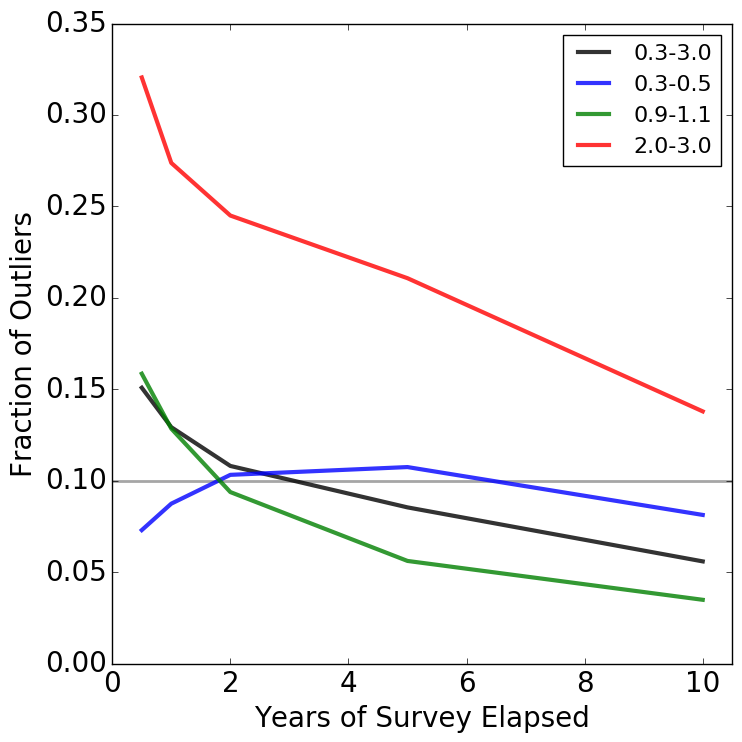
\includegraphics[width=5cm]{figs/photoz/pstat_nyears_fout.png}
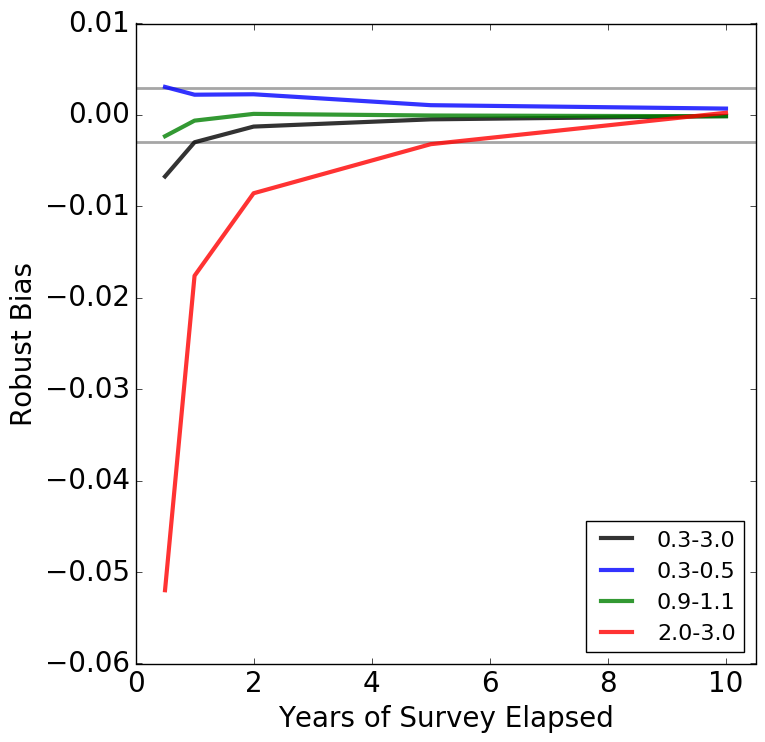
\includegraphics[width=5cm]{figs/photoz/pstat_nyears_bias.png}
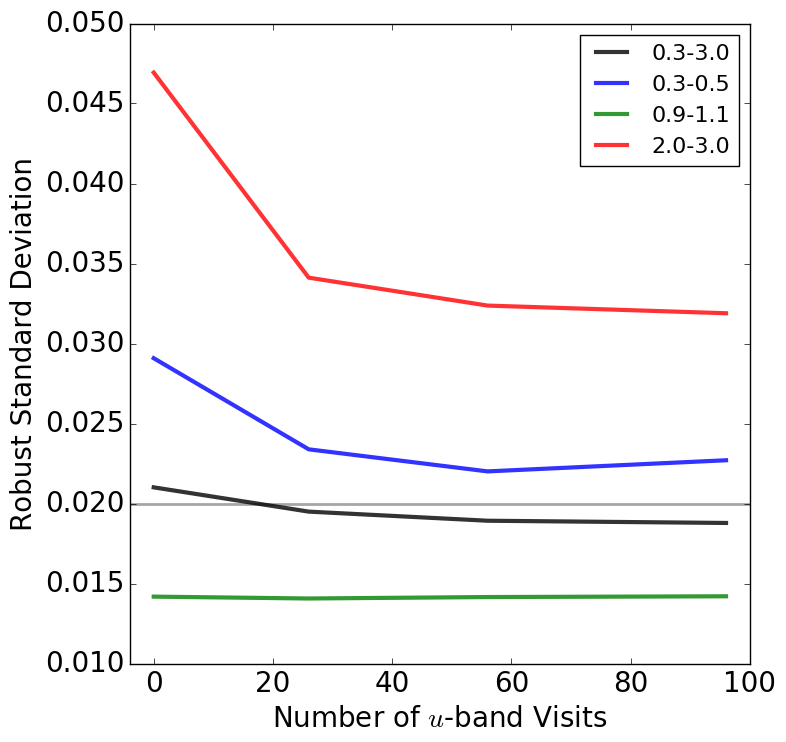
\includegraphics[width=5cm]{figs/photoz/pstat_uvisits_IQRs.png}
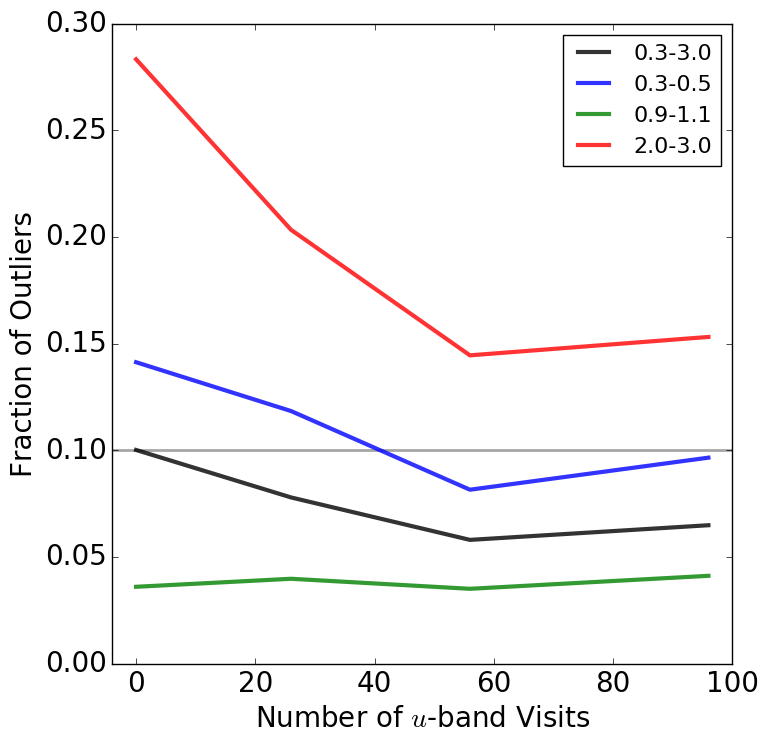
\includegraphics[width=5cm]{figs/photoz/pstat_uvisits_fout.png}
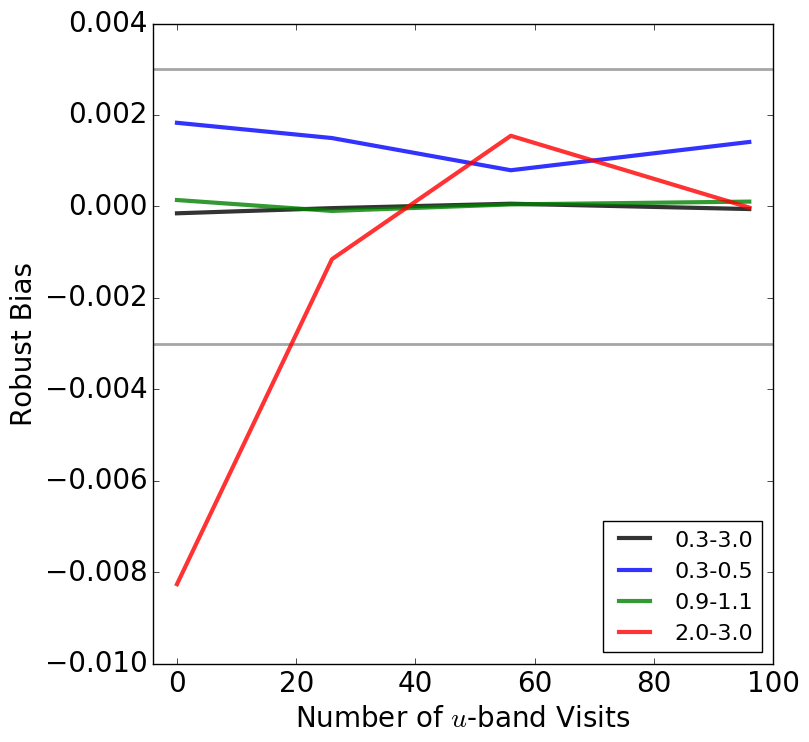
\includegraphics[width=5cm]{figs/photoz/pstat_uvisits_bias.png}
\caption{Three photo-$z$ metrics as a function of LSST parameters. From
left to right, the y-axis is the robust standard deviation, the fraction of
outliers, and the robus bias. The top row shows these statistics as a function
of the number of years of LSST survey, and the bottom row shows them as
a function of the number of $u$-band visits. Colors show these relations
for four bins in redshift: 0.3--3.0 (black), 0.3--0.5 (blue), 0.9--1.1
(green), and 2.0--3.0 (red). Grey lines mark the SRD specification for
each statistical measure.
\label{fig:metrics}}
\end{center}
\end{figure}


\subsection{Discussion}

\textbf{Additional considerations for observing strategy.} As mentioned
above, overall image depth and signal-to-noise is our primary concern,
so we are not testing changes in e.g., the inter-night gap time or the
exposure time of individual visits.  Our software is instead focused on
modifying other LSST parameters such as systematic offsets to the
magnitudes in each filter and/or coefficients for the magnitude
uncertainties in each filter in order to simulate improvements or
degradations the system throughput, sky background brightness, and other
such factors. We also aim to test airmass distributions (i.e., changes
to the effective filter functions), different progression rates for
filters (e.g., a scenario in which we complete all $u$-band by year 2),
scenarios in which some areas of sky have better/worse coverage at any
given time, and so forth. In all respects we are open to suggestions
from the community, and direct interested readers towards Graham et al. (2017; in prep.).
% Should be submitted by the end of May 2017, and then the reference can be updated.

\textbf{Considerations for building the real training catalog.} All
photometric redshift algorithms require training set data consisting of
objects with secure spectroscopic redshifts.  For LSST, many of these
will be contained in a small number of training/calibration fields (e.g.
COSMOS, VVDS).  Imaging these fields to full depth in all six bands
early in the survey (but under the range of observing conditions
expected for the ten year survey) will be key to characterizing
performance.  Inclusion of these patches of full-depth imaging must be
included in any cadence design. Future simulations of photo-$z$ results
can include varying the quality of the training catalog obtained by
LSST.

\textbf{Integration with MAF.} One way to extend our program to be able
to evaluate observing strategies simulated with \OpSim could be to use
the MAF to enable us to simulate representative samples of galaxies
across the mock LSST sky, and compute the metrics we have defined.
It may be possible to avoid such a large computation by first defining
some intermediate diagnostic metrics, such as the $u$-band coverage, and
working out how our higher level metrics depend on them, using some
approximate interpolation formulae.

\textbf{Connecting to the Dark Energy Figure of Merit.} The metrics we
have defined here should be able to be related to the DETF Figure of
Merit, but because photo-zs affect all of the LSS, WL and CL
cosmological probes, this step may need to wait until a joint
Figure of Merit MAF metric is developed.

% --------------------------------------------------------------------
%
 \subsection{Conclusions}

 Here we answer the ten questions posed in
 \autoref{sec:intro:evaluation:caseConclusions}:

 \begin{description}

 \item[Q1:] {\it Does the science case place any constraints on the
 tradeoff between the sky coverage and coadded depth? For example, should
 the sky coverage be maximized (to $\sim$30,000 deg$^2$, as e.g., in
 Pan-STARRS) or the number of detected galaxies (the current baseline but
 with 18,000 deg$^2$)?}

 \item[A1:] Since increasing the areal coverage comes at the expense of depth per pointing, this will adversely affect the photometric redshift quality. We estimate that only ~80\% of the galaxies would then meet the signal-to-noise threshold for photo-z analysis, but that this would be more than offset by the extra area and the final catalog would be ~108\% the size. Although this appears to be a net gain, it would change the redshift range for analysis.

 \item[Q2:] {\it Does the science case place any constraints on the
 tradeoff between uniformity of sampling and frequency of  sampling? For
 example, a rolling cadence can provide enhanced sample rates over a part
 of the survey or the entire survey for a designated time at the cost of
 reduced sample rate the rest of the time (while maintaining the nominal
 total visit counts).}

 \item[A2:] The sampling frequency is not important to photo-z, but building a uniform depth as a function of time would enable early science that relies on photo-z, so long as this depth is distributed across all filters. This distribution probably does not need to be exactly even, but tolerances have yet to be studied (e.g. rolling cadence may lead to seasonal variations that induce large-scale patchiness in the depth). However, sampling to full depth in all of the bands except g would have a negative impact, for example.

 \item[Q3:] {\it Does the science case place any constraints on the
 tradeoff between the single-visit depth and the number of visits
 (especially in the $u$-band where longer exposures would minimize the
 impact of the readout noise)?}

 \item[A3:] Photo-z would be improved if the u-band magnitude uncertainties could be further minimized, so long as this does not take away visits from other filters. If this could be done by longer u-band exposures during single-visits but less overall u-band visits, that would be good for photo-z.

 \item[Q4:] {\it Does the science case place any constraints on the
 Galactic plane coverage (spatial coverage, temporal sampling, visits per
 band)?}

 \item[A4:] Galactic plane coverage is not applicable to photo-z.

 \item[Q5:] {\it Does the science case place any constraints on the
 fraction of observing time allocated to each band?}

 \item[A5:] We find that at least ~20 u-band visits are necessary for the photo-z statistics to meet specifications.

 \item[Q6:] {\it Does the science case place any constraints on the
 cadence for deep drilling fields?}

 \item[A6:] Cadence of the DDF is not applicable to photo-z.

 \item[Q7:] {\it Assuming two visits per night, would the science case
 benefit if they are obtained in the same band or not?}

 \item[A7:] Intra-night filter changes do not affect photo-z.

 \item[Q8:] {\it Will the case science benefit from a special cadence
 prescription during commissioning or early in the survey, such as:
 acquiring a full 10-year count of visits for a small area (either in all
 the bands or in a  selected set); a greatly enhanced cadence for a small
 area?}

 \item[A8:] Photometric redshift analysis would be greatly assisted by acquiring a full 10-yr count of visits in all six bands for a small area during commissioning or early in the survey, especially if these assets are in regions covered by existing spectroscopic surveys.

 \item[Q9:] {\it Does the science case place any constraints on the
 sampling of observing conditions (e.g., seeing, dark sky, airmass),
 possibly as a function of band, etc.?}

 \item[A9:] Preliminary analysis shows that photometric redshifts may benefit by sampling in airmass, especially in the u-band, but a full assessment of the tradeoffs is pending. In general, a more uniform distribution of conditions is a guard against systematics.

 \item[Q10:] {\it Does the case have science drivers that would require
 real-time exposure time optimization to obtain nearly constant
 single-visit limiting depth?}

 \item[A10:] No

 \end{description}


\navigationbar

% ====================================================================


%---------------------------------------------------------------------

% ====================================================================
%+
% SECTION NAME:
%    dithering.tex
%
% CHAPTER:
%    cosmology.tex
%
% ELEVATOR PITCH:
%    Large Scale Structure, Weak Lensing, and Clusters all require
% survey uniformity in the static 10-year survey.  A key contributor to 
%this is the pattern of dithers adopted.  
%
% COMMENTS:
%
%
% BUGS:
%
%
% AUTHORS:
%   Eric Gawiser (@egawiser)
%-
% ====================================================================
\clearpage
\section{Large Scale Structure:  Testing Dithering Patterns and Timescales to Improve Survey Uniformity}
\def\secname{dithering}\label{sec:\secname}

\noindent{\it Humna Awan, Eric Gawiser, Peter Kurczynski, Lynne Jones} % (Writing team)

% This individual section will need to describe the particular
% discoveries and measurements that are being targeted in this section's
% science case. It will be helpful to think of a ``science case" as a
% ``science project" that the authors {\it actually plan to do}. Then,
% the sections can follow the tried and tested format of an observing
% proposal: a brief description of the investigation, with references,
% followed by a technical feasibility piece. This latter part will need
% to be quantified using the MAF framework, via a set of metrics that
% need to be computed for any given observing strategy to quantify its
% impact on the described science case. Ideally, these metrics would be
% combined in a well-motivated figure of merit. The section can conclude
% with a discussion of any risks that have been identified, and how
% these could be mitigated.

% A short preamble goes here. What's the context for this science
% project? Where does it fit in the big picture?

Three of the key cosmology probes available with LSST represent ``static science'' insensitive to time-domain concerns.  These are Weak Lensing, Large-Scale Structure, and Galaxy Clusters.  Nonetheless, due to the need to track and correct for the survey ``window function'' in all of these probes, cosmology with LSST will benefit greatly from achieving survey depth as uniform as possible over the WFD area.  OpSim tiles the sky in hexagons inscribed within the nearly-circular LSST field-of-view.  It has been shown in \citet{CarrollEtal2014} that the default LSST survey strategy implemented in OpSim runs leads to a strongly non-uniform ``honeycomb'' pattern due to overlapping regions on the edges of these hexagons receiving double the observing time.  A pattern of large dithers proves sufficient to greatly reduce these overlaps, leading to an increase in median survey depth in each filter of 0.08 magnitudes.  

In this section, we report results from an investigation by Awan et al. (in preparation) of several geometrical patterns for dithers performed on timescales varying from once per observing season to once per night to every visit.  

\todo{EG}{Flesh out WL, LSS, and Clusters dependence on survey uniformity to make this section more clearly science-driven.}  

% --------------------------------------------------------------------

\subsection{Dithering Patterns and Timescales}
\label{sec:\secname:strategies}


% --------------------------------------------------------------------

\subsection{Metrics}
\label{sec:\secname:metrics}

% Quantifying the response via MAF metrics: definition of the metrics,
% and any derived overall figure of merit.

Our primary metric is total uncertainty in the derived window function over relevant angular scales, modeled via variations in the angular power spectrum of fake galaxy fluctuations between $gri$ bands.  
Intermediate metrics include the number of galaxies in 
each pixel, fluctuations in this number, total power in the angular power spectrum of a skymap of those fluctuations, and residual power that angular power spectrum after subtracting a smooth fit to it.  



% --------------------------------------------------------------------

\subsection{OpSim Analysis}
\label{sec:\secname:analysis}

% OpSim analysis: how good would the default observing strategy be, at
% the time of writing for this science project?

In this section we present our ongoing \OpSim / MAF
analysis, as we try to
answer the question ``what dithering strategies produce acceptable variations in survey uniformity, and which appears optimal?''

%We used the
%\simsMAFcontrib{SeasonStacker}{mafContrib/seasonStacker.py} to work
%with seasons.

%We used \texttt{ops2\_1075} for most of our tests, but we need to now
%re-run on \opsimdbref{db:enigma}, and others from \autoref{chp:cadence2015}.


%\citeauthor{LiaoEtal2015}). These sky maps show that, over the main

%\autoref{tab:lenstimedelays:results} shows the global (i.e. al-sky)


%--------------------------------------------------------------------

\subsection{Results}
\label{sec:\secname:results}


\todo{EG}{Improve figures to originals rather than screen-captures.}


%%%%%%%%%%%%%%%%%%%%%%%%%%%%%%%%%
\begin{figure}[tbh!]
\vskip -0.1in
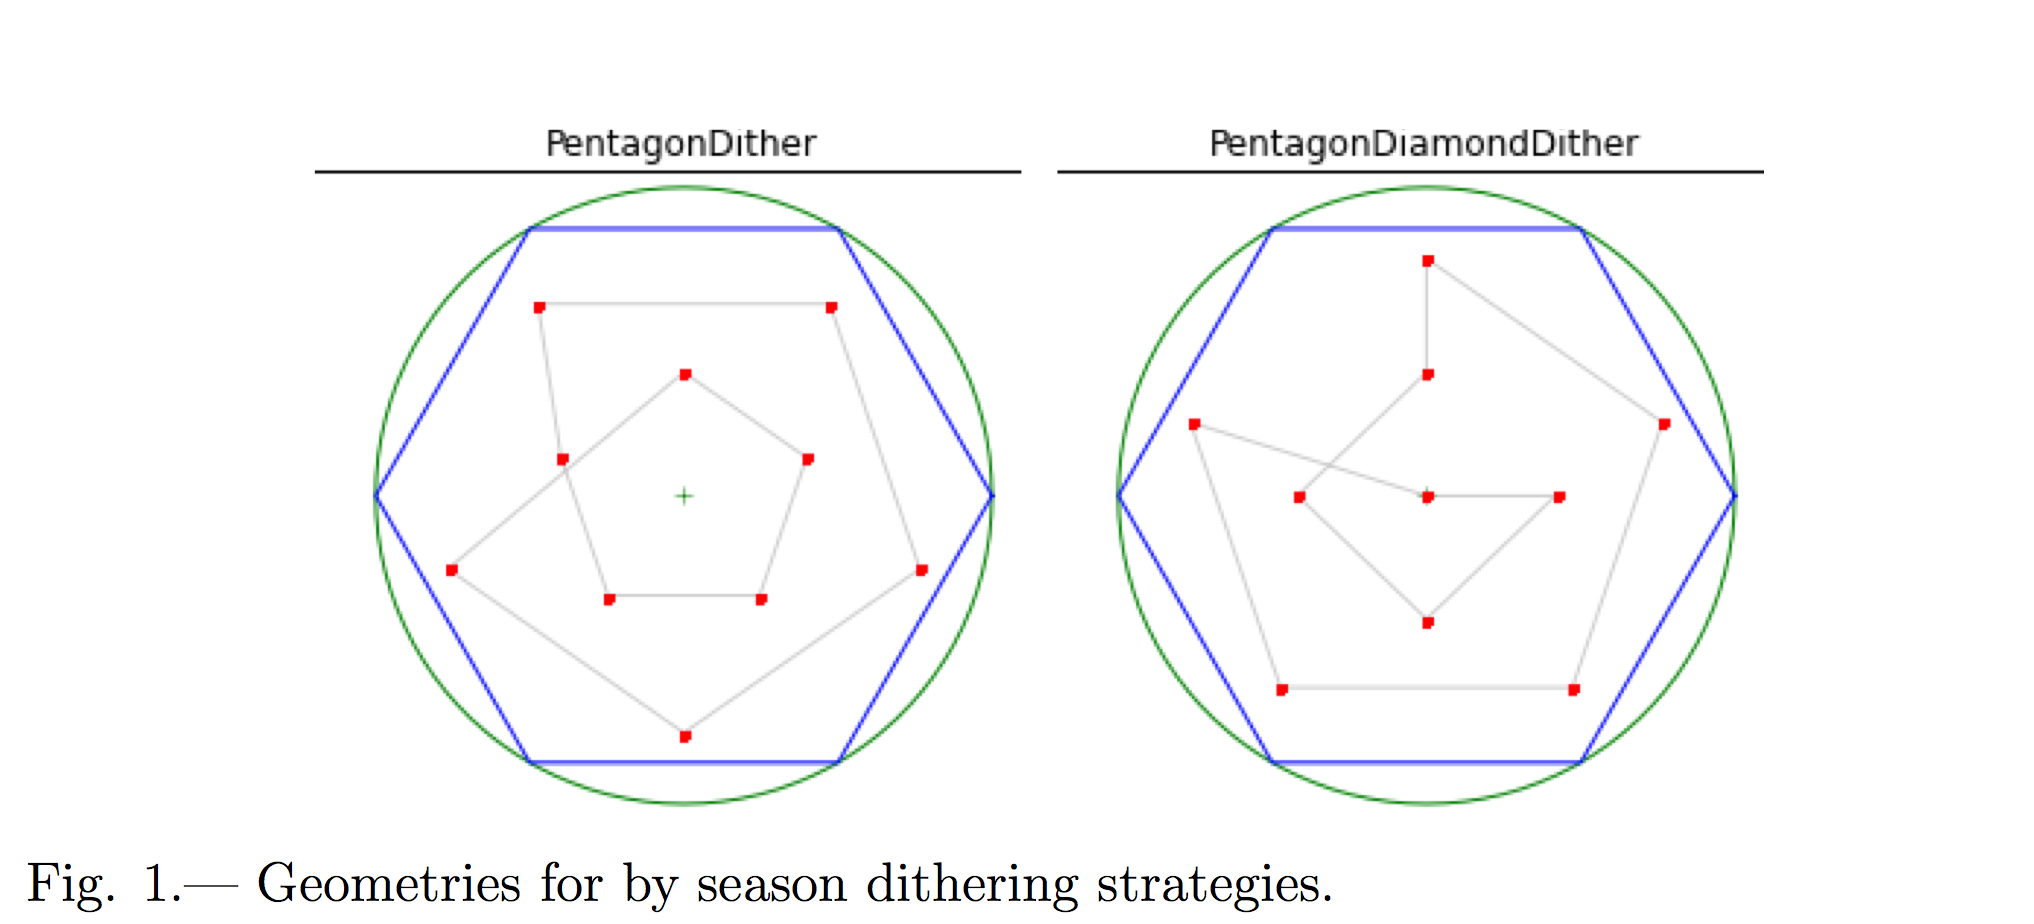
\includegraphics[angle=0,width=0.99\hsize:,clip]{figs/awan_fig1.png}
%\vskip -1.3in
\caption{}
\label{fig:seasonal_dithers}
\end{figure}
%%%%%%%%%%%%%%%%%%%%%%%%%%%%%%%%%

%%%%%%%%%%%%%%%%%%%%%%%%%%%%%%%%%
\begin{figure}[tbh!]
\vskip -0.1in
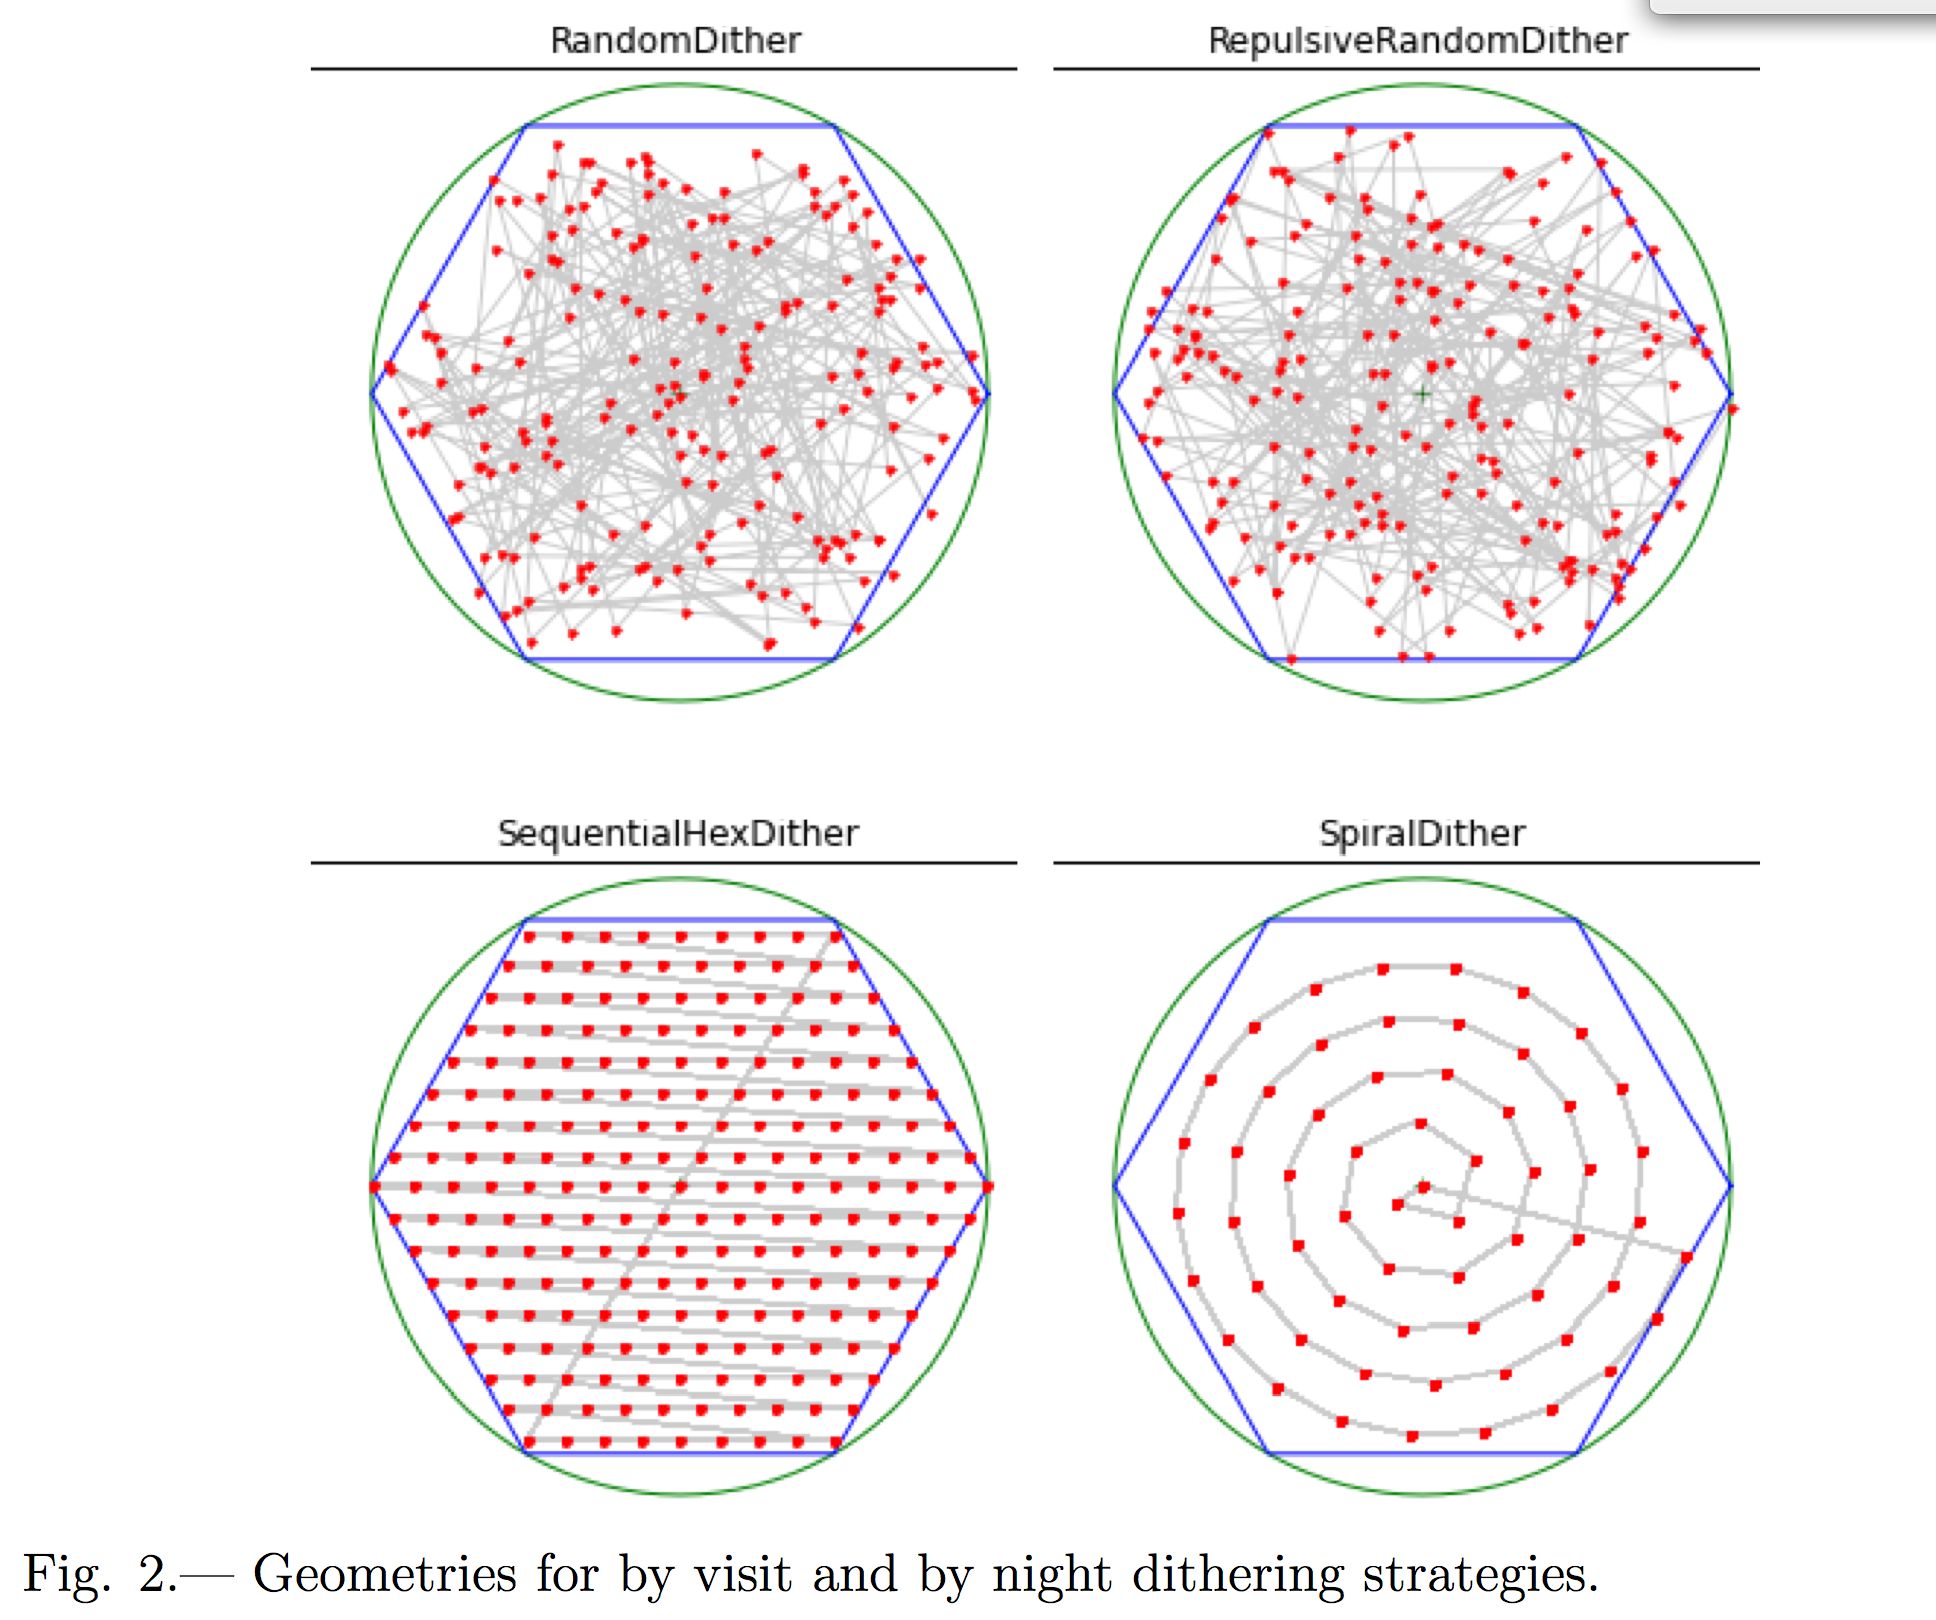
\includegraphics[angle=0,width=0.99\hsize:,clip]{figs/awan_fig2.png}
%\vskip -1.3in
\caption{}
\label{fig:nightly_dithers}
\end{figure}
%%%%%%%%%%%%%%%%%%%%%%%%%%%%%%%%%

%%%%%%%%%%%%%%%%%%%%%%%%%%%%%%%%%
\begin{figure}[tbh!]
\vskip -0.1in
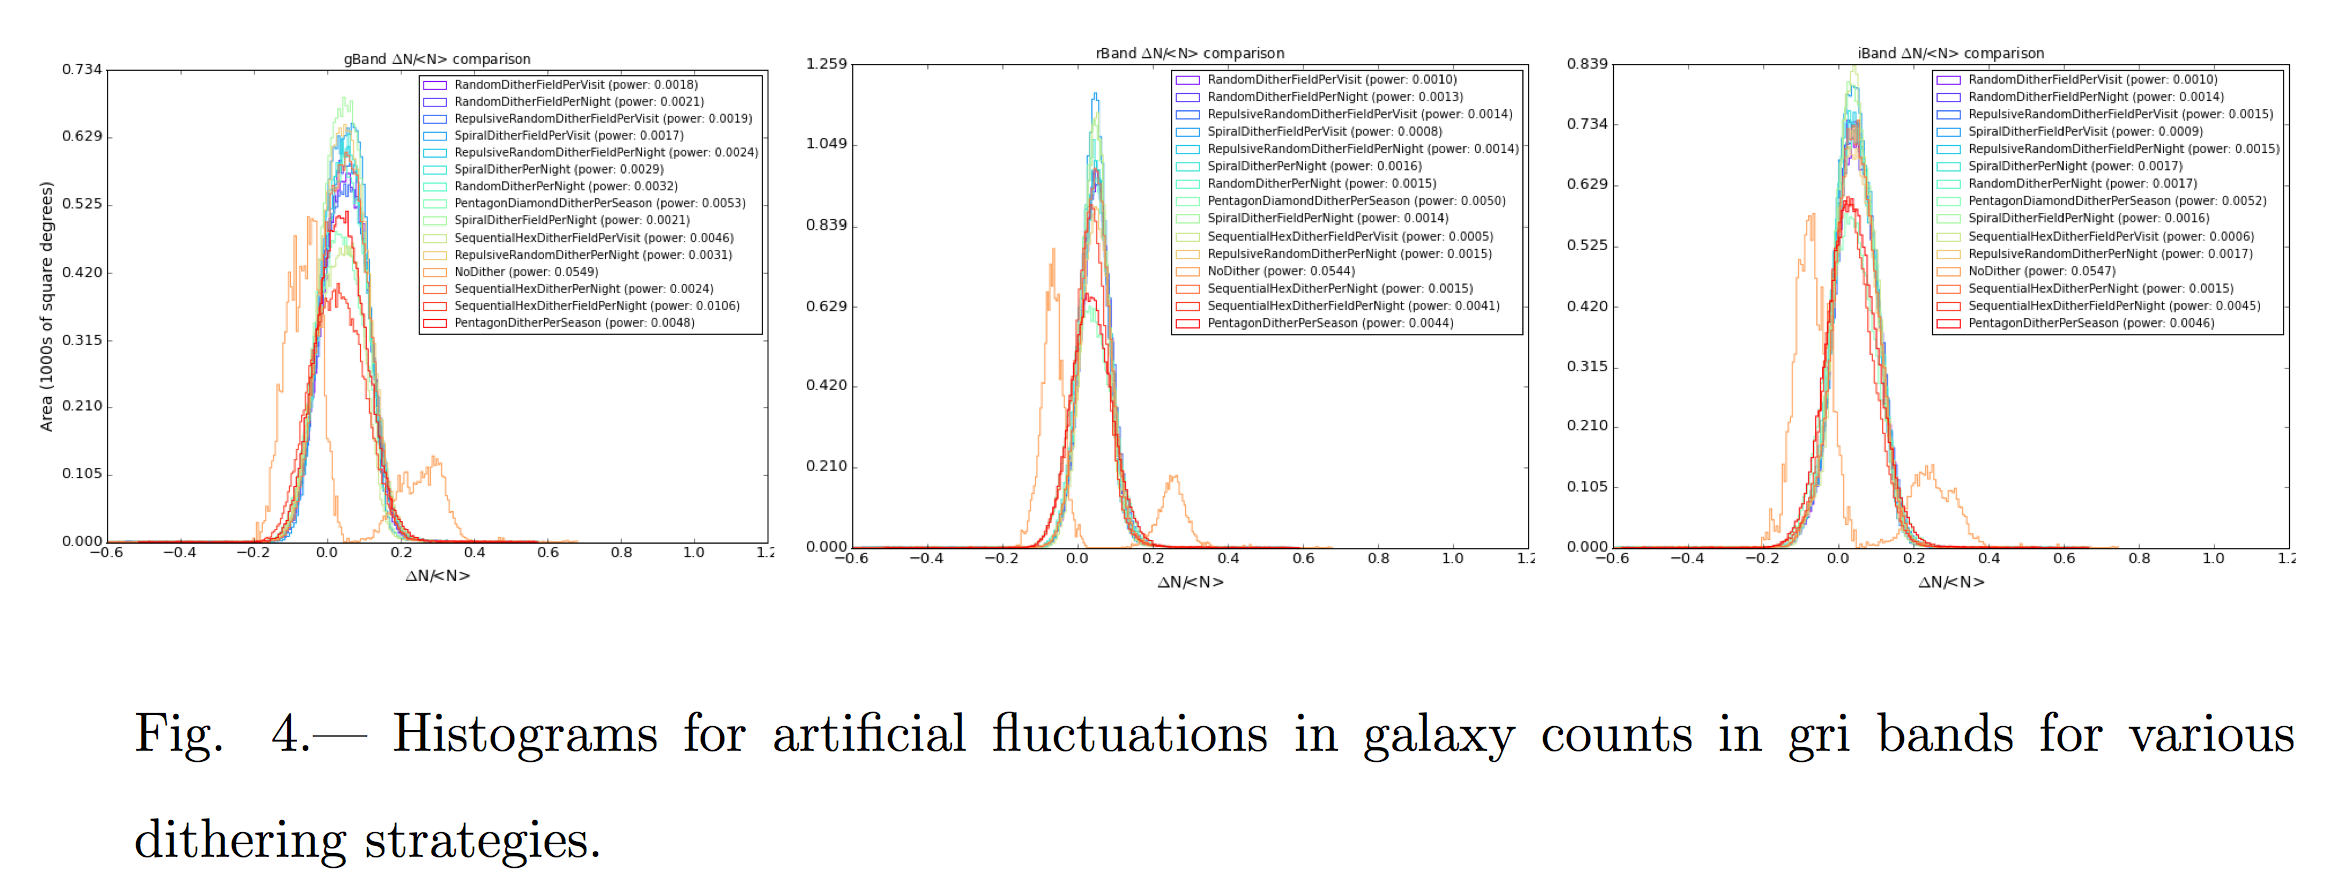
\includegraphics[angle=0,width=0.99\hsize:,clip]{figs/awan_fig4.png}
%\vskip -1.3in
\caption{}
\label{fig:dithering_histograms}
\end{figure}
%%%%%%%%%%%%%%%%%%%%%%%%%%%%%%%%%

%%%%%%%%%%%%%%%%%%%%%%%%%%%%%%%%%
\begin{figure}[tbh!]
\vskip -0.1in
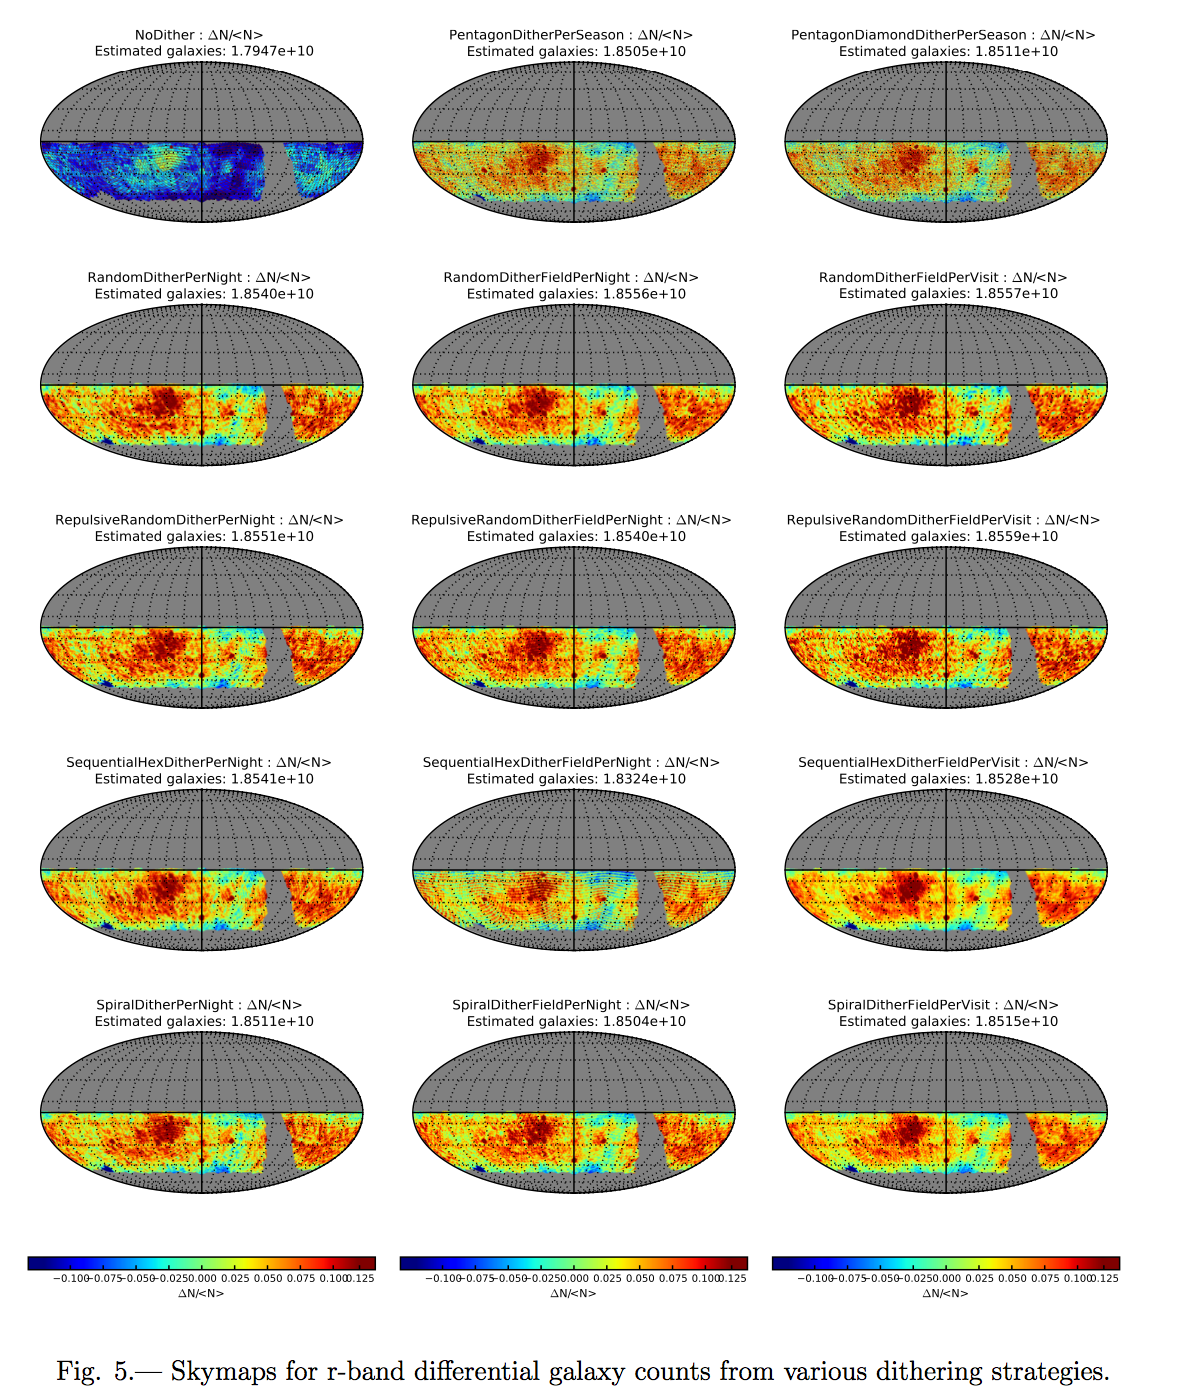
\includegraphics[angle=0,width=0.99\hsize:,clip]{figs/awan_fig5.png}
%\vskip -1.3in
\caption{}
\label{fig:dithering_skymaps}
\end{figure}
%%%%%%%%%%%%%%%%%%%%%%%%%%%%%%%%%

%%%%%%%%%%%%%%%%%%%%%%%%%%%%%%%%%
\begin{figure}[tbh!]
\vskip -0.1in
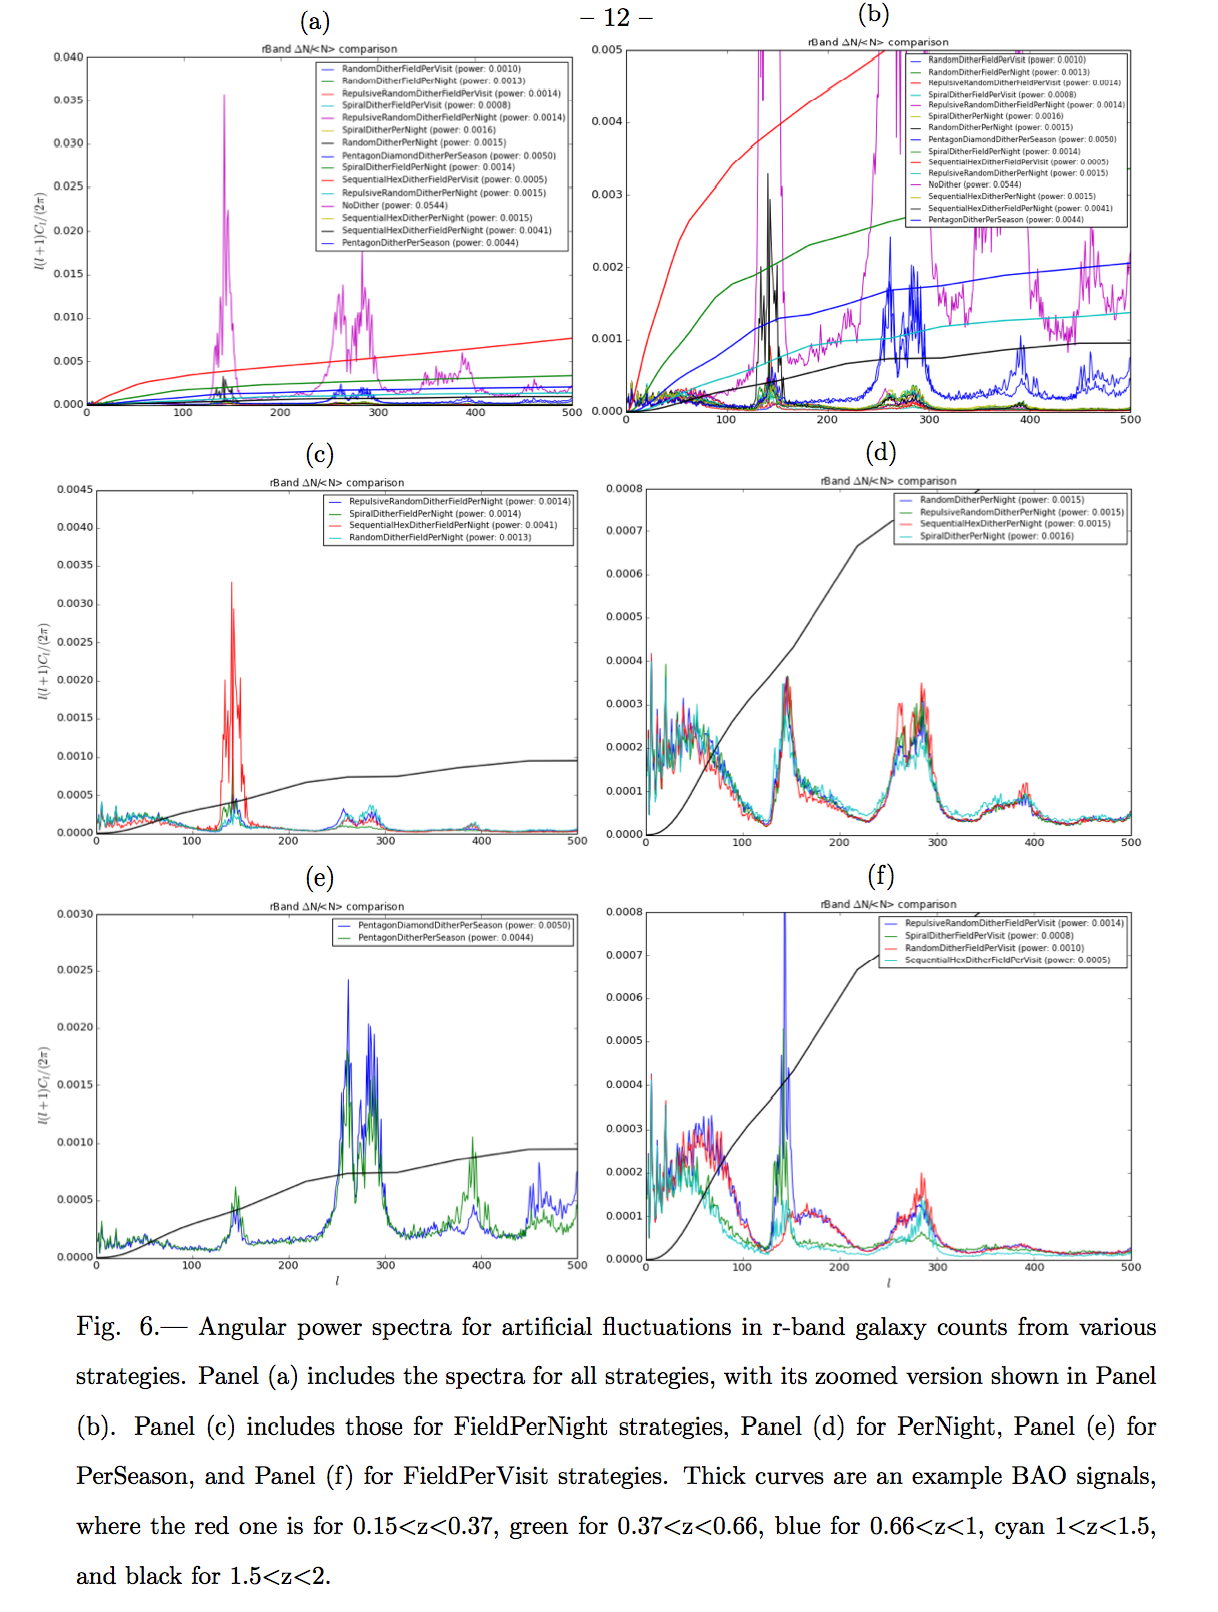
\includegraphics[angle=0,width=0.99\hsize:,clip]{figs/awan_fig6.png}
%\vskip -1.3in
\caption{}
\label{fig:dithering_power_spectra}
\end{figure}
%%%%%%%%%%%%%%%%%%%%%%%%%%%%%%%%%




%%%%%%%%%%%%%%%%%%%%%%%%%%%%%%%%%%%%
%\begin{figure*}[!ht]
%  \capstart
%  \begin{minipage}[b]{\linewidth}
%    \begin{minipage}[b]{0.32\linewidth}
%      \centering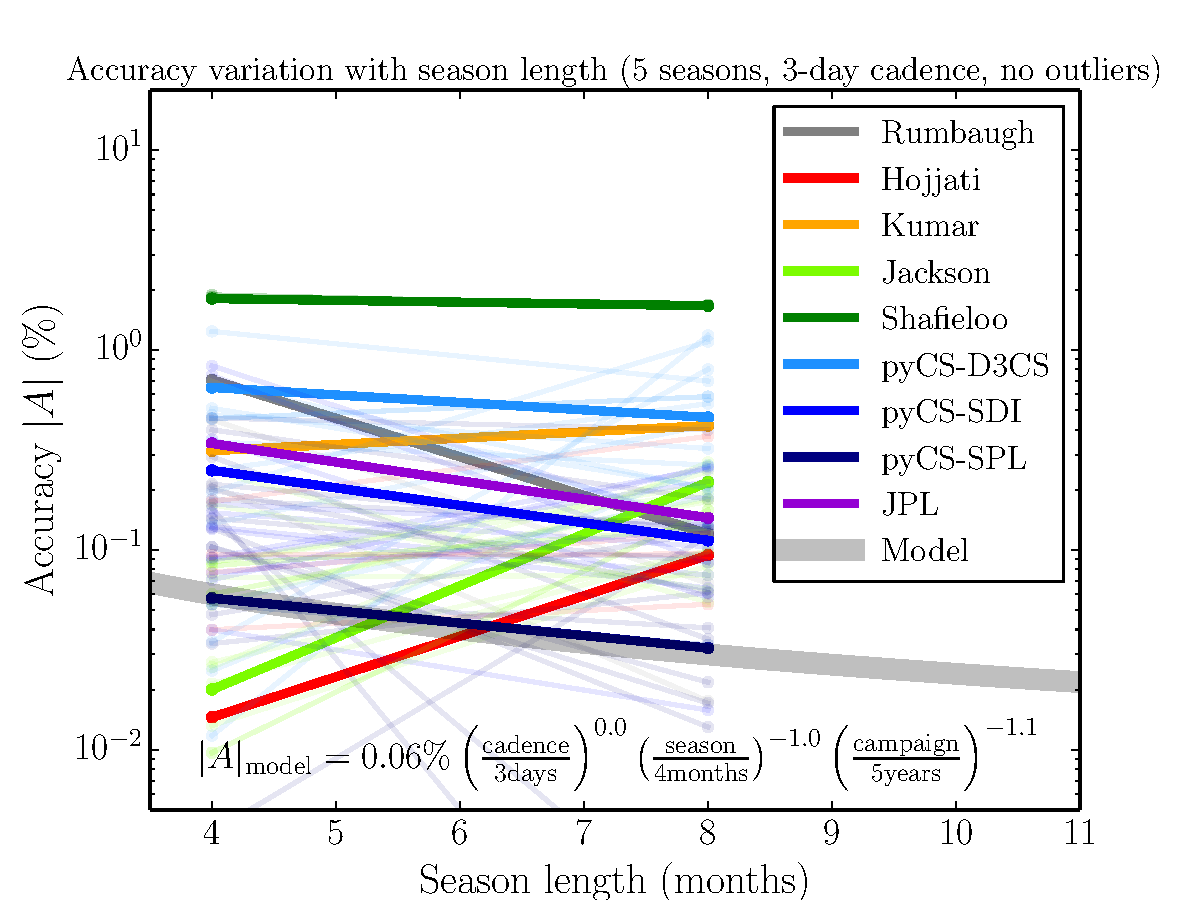
\includegraphics[width=\linewidth]{figs/Accuracy_season_nca.pdf}
%    \end{minipage} \hfill
%    \begin{minipage}[b]{0.32\linewidth}
%      \centering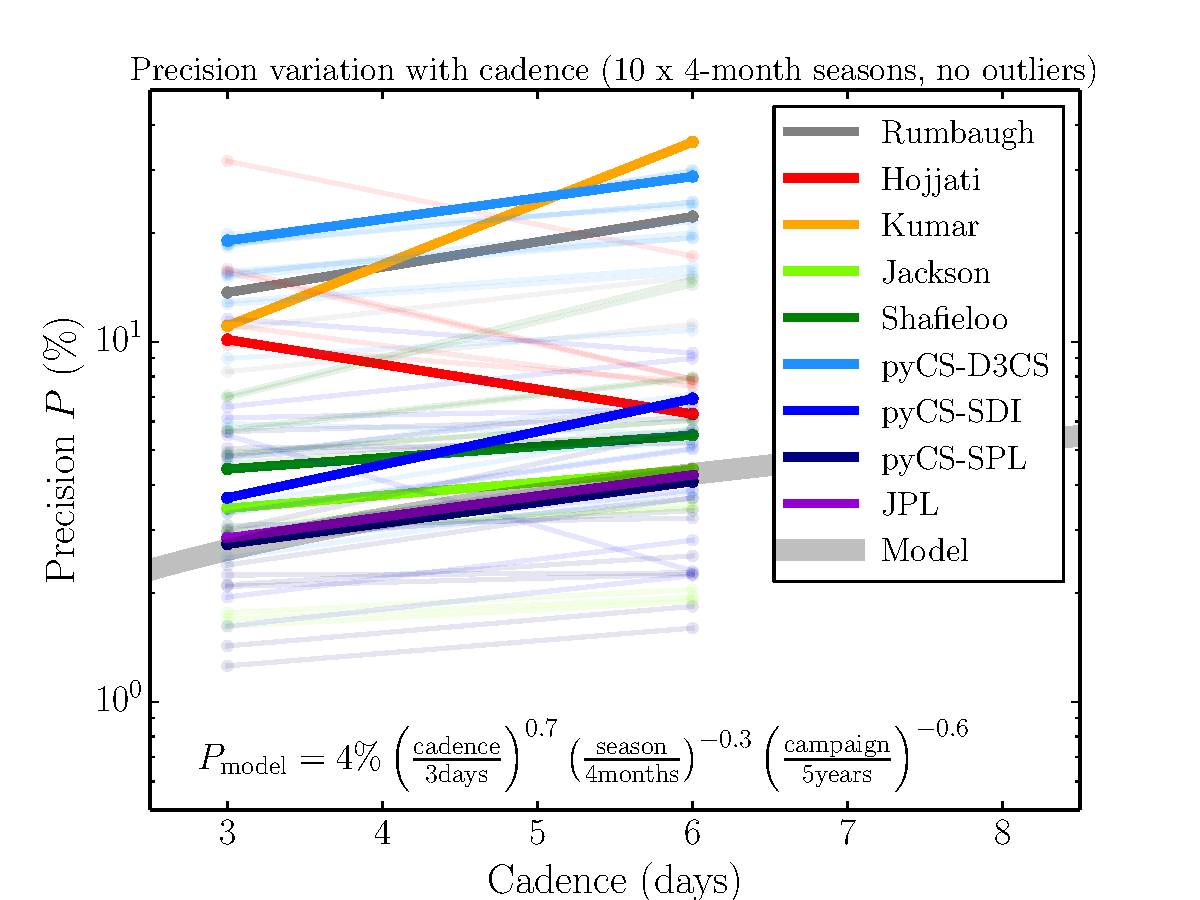
\includegraphics[width=\linewidth]{figs/Precision_cadence_nca.pdf}
%    \end{minipage} \hfill
%    \begin{minipage}[b]{0.32\linewidth}
%      \centering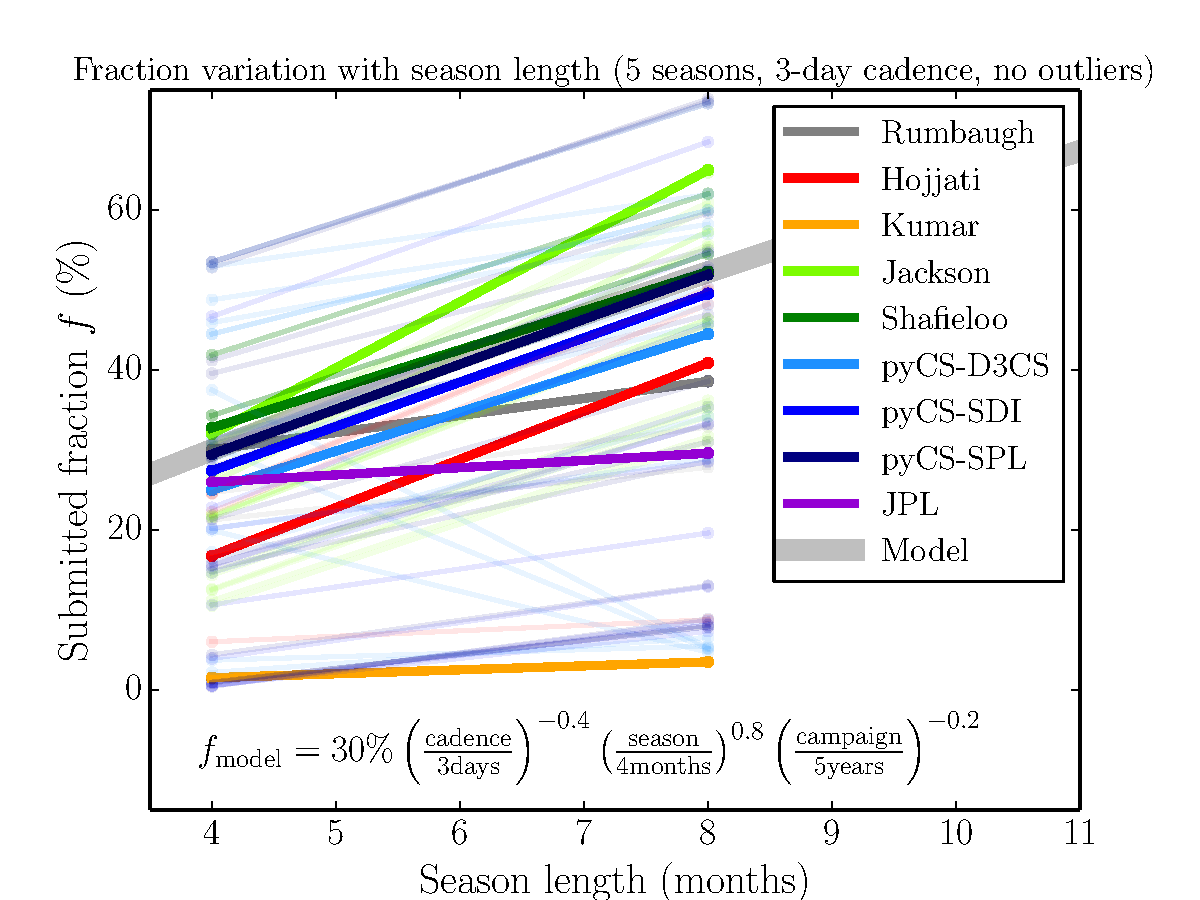
\includegraphics[width=\linewidth]{figs/Fraction_season_nca.pdf}
%    \end{minipage}
%  \end{minipage}
%\caption{Examples of changes in accuracy $A$ (left), precision $P$ (center) and success fraction $f$ (right) with schedule properties, as seen in the different TDC submissions. The gray
%approximate power law model was derived by visual inspection of the
%pyCS-SPL results; the signs of the indices were pre-determined according to our expectations. Reproduced from \citet{LiaoEtal2015}.}
%\label{fig:tdcresults}
%\end{figure*}
%%%%%%%%%%%%%%%%%%%%%%%%%%%%%%%%%%%


\todo{EG}{Input fuller results and text from Awan et al. draft.}  

%---------------------------------------------------------------------

\subsection{Discussion}
\label{sec:\secname:discussion}



\navigationbar

% ====================================================================


% --------------------------------------------------------------------


\section{Suppressing systematic effects}

Much of cosmology science may be limited by systematic errors rather than photon signal-to-noise.  

\subsection{Target Measurements}

It is expected that even after maximal optimization of camera optics and electronics, that systematic image shape errors will be associated with the orientation of the camera focal plane.  These can be partially reduced by randomization of the orientation of the camera with respect to the sky.  This is represented by the parameter RotSkyPos.  

Similarly, the telescope optics may harbor systematic aberrations, and these also could be mitigated by recording images with varying parallactic angle.  Another relevant parameter, RotTelPos, is indicative of the projected angle of the telescope optics on the sky.  


\subsection{Metrics}

A metric is available for RotSkyPos.  The metric computes, for any selected filter and simulation, a histogram of the distribution of rms values of RotSkyPos computed per field. It also computes basic statistics of these distributions.

\subsection{OpSim Analysis}


\begin{figure}
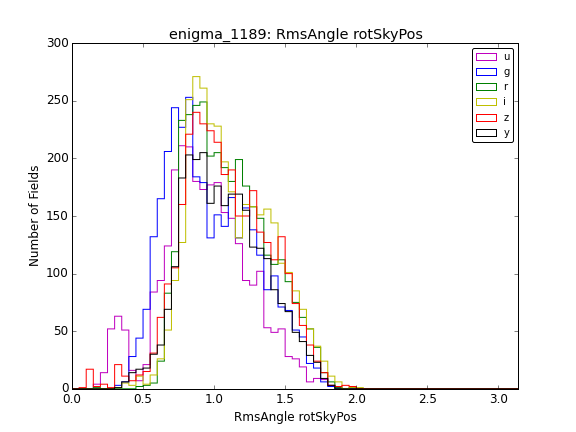
\includegraphics[width=5.0in]{enigma1189RmsAnglerotSkyPosugrizybandallpropsOPSIComboHistogram.png}
\caption{The relative angle of the detector plane with respect to the sky, RotSkyPos, as a histogram showing the number of fields vs. rms of the parameter.}
\label{RotSkyPos}
\end{figure}

The distribution of rms values by filter is shown in Figure \ref{RotSkyPos} for the current candidate baseline simulation, enigma\_1189.  As shown, the rms values cluster around the value 1 radian,  with typical values 1 +- 0.3 radian.  This compares to a completely uniform distribution over the half circle with an rms of 1.14.  

\subsection{Discussion}

The RotSkyPos metric analysis shows that the majority of fields have a good randomization of detector angles projected on the sky.

There are several limitations to this observation.

First, we do not have at present a quantitative requirement for randomization of this parameter.  In future development of weak lensing analysis, a criterion should be developed.

Second, a significant fraction of fields  have median values that are lower or higher than expected for a random distribution, with some far from uniformly distributed.  Regardless of the $per field$ criterion, it is desirable to avoid the incidence of individual discrepant fields.

The recommended criterion for randomization of RotSkyPos is not the behavior of the majority of the fields, but of the minority with the least random behavior.  The number of non-random fields should be minimized.  A recommended metric is the count of fields with median RMS less then 0.8 or greater than 1.5 radians (these values to be reviewed again as additional experience is gained with additional OpSim schedule simulations and weak lensing analysis.)

A similar metric for RotTelPos should be developed. Other observing parameters may benefit from randomization, but are not presently recommended for metric analysis.


% --------------------------------------------------------------------

% ====================================================================
%+
% SECTION:
%    supernovacosmology.tex
%
% CHAPTER:
%    cosmology.tex
%
% ELEVATOR PITCH:
%    SNIa cosmology, approach to evaluating dependence of science on cadence
%
% COMMENTS:
%
%
% BUGS:
%
%
% AUTHORS:
%    Phil Marshall (@drphilmarshall)  - put your name and GitHub username here!
%-
% ====================================================================

\section{Supernova Cosmology and Physics}
\def\secname{supernovae}\label{sec:\secname}
% \label{sec:cosmology, supernovae, classification, lenstimedelays, deepdrillingfields }

\noindent{\it Jeonghee Rho, Michelle Lochner, Rahul Biswas} % (Writing team)

% This individual section will need to describe the particular
% discoveries and measurements that are being targeted in this section's
% science case. It will be helpful to think of a ``science case" as a
% ``science project" that the authors {\it actually plan to do}. Then,
% the sections can follow the tried and tested format of an observing
% proposal: a brief description of the investigation, with references,
% followed by a technical feasibility piece. This latter part will need
% to be quantified using the MAF framework, via a set of metrics that
% need to be computed for any given observing strategy to quantify its
% impact on the described science case. Ideally, these metrics would be
% combined in a well-motivated figure of merit. The section can conclude
% with a discussion of any risks that have been identified, and how
% these could be mitigated.

This section is concerned with the detection and characterization of supernovae (SNe)
over time with LSST and their various scientific applications.
The most important
application is the use of supernovae type Ia (SNIa) and potentially some core-collapse SN (like type IIP) to trace the recent expansion history of the universe,
and confront models of the physics driving the late time accelerated expansion
of the universe. 

This objective of SN cosmology follows (at least for SNIa) results from several
highly successful surveys; improvement in knowledge of SN cosmology could come from
substantially larger numbers of well-characterized SNe and potentially
useful redshift distributions of such detected SNe. In this sense, this
goal is not directly tied to the unprecedentedly large survey area of LSST.  
However, we shall argue that in practice, even this
goal would benefit from the spatial scale offered by the Wide Fast Deep
(WFD) component of the LSST survey. 

On the other hand, the WFD component of the LSST survey is potentially the 
first single survey to scan for SNe across the very large area of the
entire Southern sky.  SNe that are detected and well characterized by LSST will
probe the isotropy of the universe.  Peculiar velocities of 
SNe will probe the growth of structure.  In addition, this large sample
will enable further
sharpening of our understanding of the properties of the supernova population 
of different types. 
This last point is extremely important for SN cosmology goals:  The success of SNIa cosmology has always been based on the empirical model that intrinsic peak brightnesses are related to the certain observable characteristics of SNe. 
%While the spatial locations of the SNe are not important
The 
WFD has the potential to dramatically increase the size of the sample 
available to train such an empirical model, as well understand the probability of deviations and scatter from this model. Aside from issues like calibration 
which need to be addressed differently, a larger sample of such well measured SNe is probably the only way to address `systematics' due to deviations from the empirical
model. The anticipated sample can be thought of as consisting of two 
components:  the low-redshift sample which is more likely to be complete, and the higher-redshift sample that will be able to constrain evolution. 
% --------------------------------------------------------------------

\subsection{Target measurements and discoveries}
\label{sec:keyword:targets}

% Describe the discoveries and measurements you want to make.

SNe of different types are visible over time scales of about a few 
weeks (e.g., type Ia) to nearly a year (type IIP).  During the full ten-year
 survey, LSST will scan the entire southern sky repeatedly
 with a WFD cadence, and certain specific locations
of the sky called the Deep Drilling Fields (DDF) with special enhanced cadence. 

This spatio-temporal window should contain millions (RB: remember to check) of SNe, that will have apparent magnitudes brighter than the single exposure limiting magnitude of LSST.  However, the actual
 sequence of observations by LSST, defined by the series of field pointings as a
 function of time in filter bands (along with weather conditions) will
 determine the extent to which each SN can be detected and
 characterized well.  Characterization of the SNe is at the core of a
 number of science programs that use them as bright, abundant objects with empirically determined intrinsic brightness. For LSST, this goal entails (a) detection of SNe, (b) photometric typing of SNe, (c) estimating photometric redshifts of SNe (or identifying host galaxies 
 and obtaining their redshifts from photometry or follow-up spectroscopy),
(d) estimation of intrinsic brightnesses of the SNe, and finally use of these data in addressing our science goals of cosmological inference, etc.
The efficacy of photometric typing, redshifts and estimation of intrinsic brightnesses are all
dependent on the amount of information available in the observed light curves of SNe. While these steps are not necessarily independent, it is useful to think of the requirements on some of these steps separately; it is not unlikely  that combining some of these steps would still be affected by similar requirements. 

{\emph{Our first objective is to detect such SNe}}, by which we mean
selecting SNe from among the transient sources detected by LSST.
% classify them as SNe (as opposed to an AGN, or an asteroid). 
In brief, this process 
consists of defining a set of image subtractions between high 
resolution `template` image of a sky section, and a set of single exposures at
different times (usually of lower resolution) of the same region, after 
accounting for the different resolutions of images, and alignments. These sets of image subtractions associated
 with a single object will be used to detect the object as a transient and then
classify the transient as an SN. Clearly, detecting an SN depends on the number of such images recorded per object, the number of filters, and the signal-to-noise ratios of the images. %One might expect that 
The efficiency of this step may be summarized as a threshold on the joint properties 
of an astrophysical candidate (apparent brightness, light curve characteristics, background) as well as observing conditions (astronomical seeing, etc.).  

{\emph{Our second objective is to photometrically classify different kinds of SNe.}} 
%{\bfseries Photometric SN classification}\\
Previously, only spectroscopically typed SNe have been used for cosmology. Photometric 
typing from light curves alone has only been used to select candidates for spectroscopic 
follow-up (see, e.g., \citet{Sako2008}). However, LSST will simply find far too many 
candidates for even a significant fraction of them to be followed up spectroscopically. In order to avoid 
discarding the majority of the SN dataset, we need to use techniques capable of 
determining cosmological parameters from a potentially contaminated photometric SN dataset.

Several techniques have been proposed in recently to solve this problem. One 
approach proposes applying stringent cuts to the photometric dataset to obtain a nearly pure sample 
of SNIa\citep{Bernstein2012,Campbell2013} and to run the standard SNIa cosmology analysis 
with this sample. Another approach, BEAMS \citep{Kunz2007,Newling2011,Hlozek2012,Knights2013}, 
makes use of an entire dataset, coping with contamination by using a mixture model for the 
likelihood, thus allowing for multiple populations. Whatever the technique ultimately used for 
cosmological analysis, it will rely on accurate initial classifications of SN type and 
unbiased estimates for the probability of each type.

Current state-of-the-art photometric classification techniques rely on fitting empirically 
determined templates of SNe to light curves \citep{Jha2007,Guy2007,Sako2011}. However in 
recent years, new approaches have been developed in response to the 2010 `Supernova 
Photometric Classification Challenge' \citep{Kessler2010a}. Many of these use novel light curve 
parameterization and employ machine learning algorithms to perform the classification (see \citet{Kessler2010b} and references therein).

While many of these methods have been tested on standard sets of simulated data and (in some cases) 
on SDSS data, which technique (if any) is superior in all situations is unclear. For 
example, some techniques are dependent on the availability of reliable redshift information. 
%, while others  are less reliant on it. 
Some techniques may be more robust to non-representative datasets [Not sure what this means] than 
others, and how the techniques will respond to changes in cadence, filter sets, signal-to-noise, 
etc., is unclear.  

With this in mind, we propose the use of a multifaceted classification system which employs 
several different methods for extracting features from the light curves (e.g., fitting parametric 
functions or templates) and several different classification algorithms. This system is highly 
modular, allowing new approaches for direct comparison with existing  techniques to be added easily. This also allows direct analysis of different observing strategies, without requiring 
an initial choice of classification technique. 


{\emph{Our third objective is to characterize SNe in terms of empirical
    light curve models.}}

The ultimate goal of using SNe (type SNIa or SNIIP) for cosmology requires estimating their intrinsic brightnesses of the supernova. The
first (and sometimes only, depending on the light curve model) step is
fitting the calibrated fluxes to a light curve model with a set of parameters.
According to the ansatz used in SN cosmology, the intrinsic brightness of
 SNe is largely determined by the parameters of the light curve model; 
 hence the uncertainties on the inferred parameters largely determine the
 uncertainties on the inferred peak intrinsic brightness or distance moduli of the SNe.

% Now, describe their response to the observing strategy. Qualitatively,
% how will the science project be affected by the observing schedule and
% conditions? 

% In broad terms, how would we expect the observing strategy
% to be optimized for this science?





% --------------------------------------------------------------------

\subsection{Metrics}
\label{sec:keyword:metrics}

Quantifying the response via MAF metrics: definition of the metrics,
and any derived overall figure of merit.

\emph{To be added: discussion of the ROC curve as a useful metric for photometric supernova 
classification}




% --------------------------------------------------------------------

\subsection{OpsSim Analysis}
\label{sec:keyword:analysis}

OpSim analysis: how good would the default observing strategy be, at
the time of writing for this science project?

As noted above the scientific goal of characterizing SNe is to a large extent
dependent on how well the light curves of individual SNe are sampled in
time and filters. To study this, we re-index the OpsSim output on spatial
locations rather than use the temporal index. There are different methods (which will be merged), and here we will first illustrate this in terms the cadence in an example LSST field.

\begin{figure}
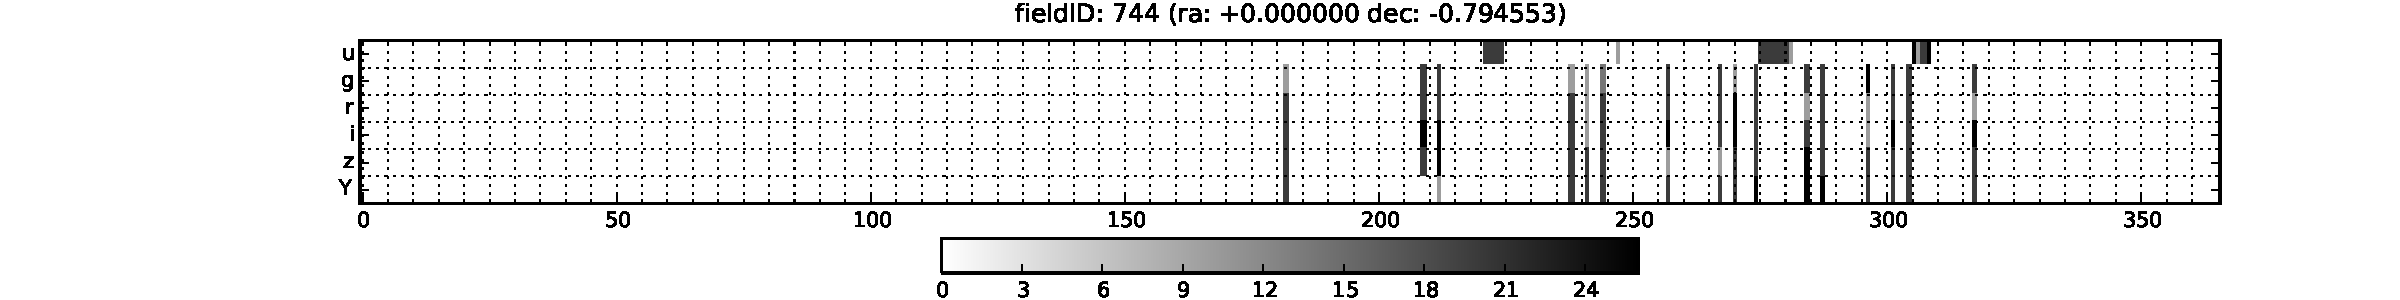
\includegraphics[width=\textwidth]{figs/supernova/fig_firstSeason_0}
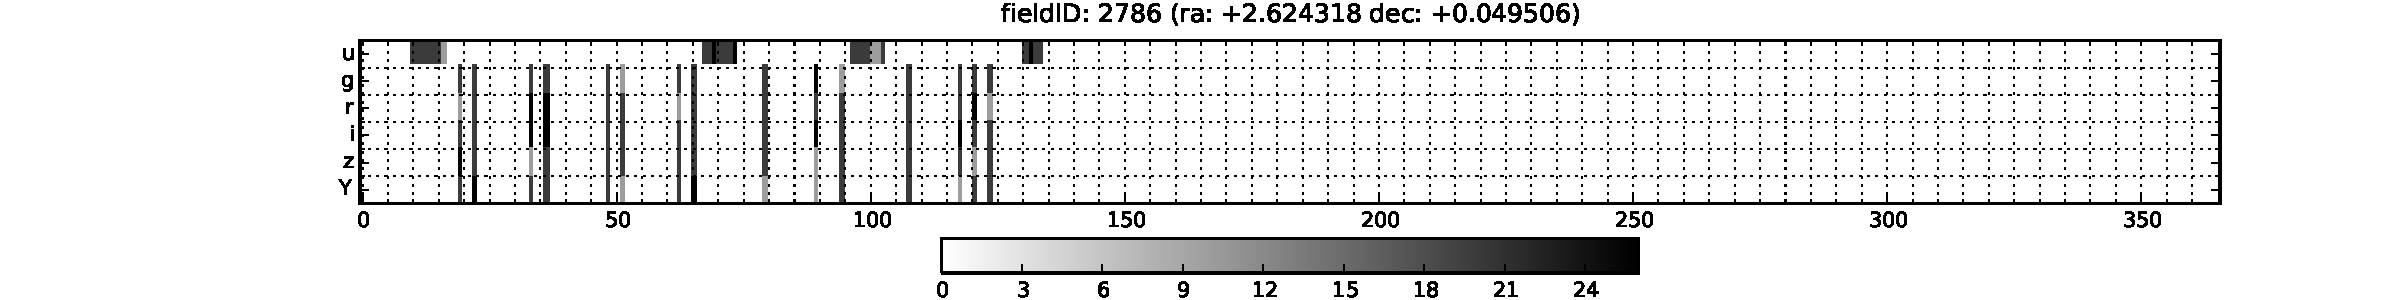
\includegraphics[width=\textwidth]{figs/supernova/fig_firstSeason_1}
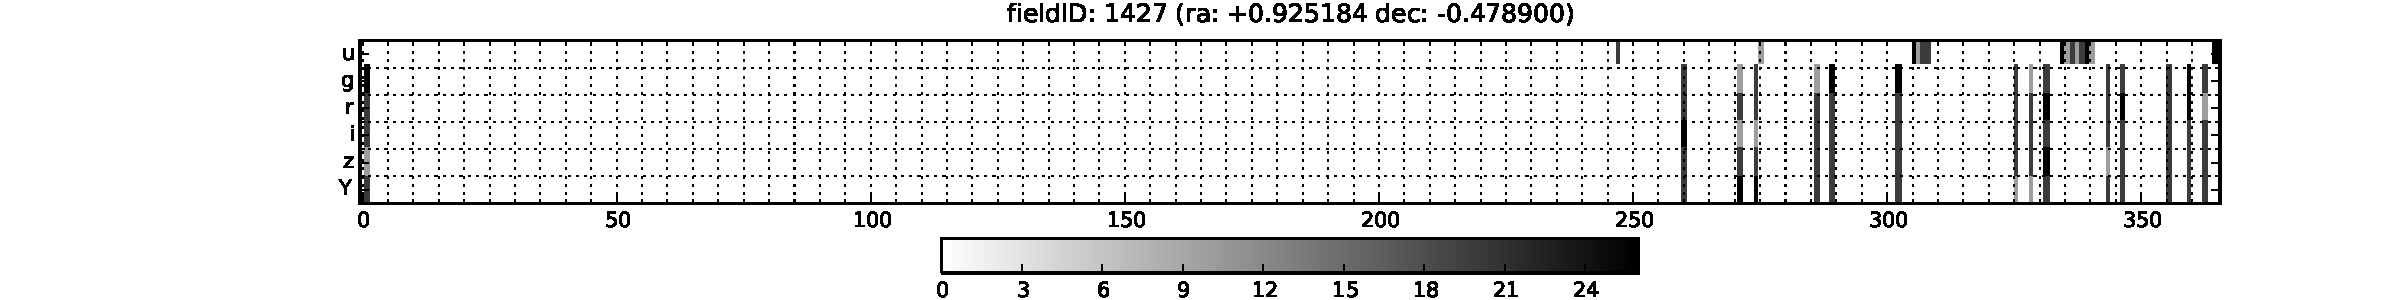
\includegraphics[width=\textwidth]{figs/supernova/fig_firstSeason_2}
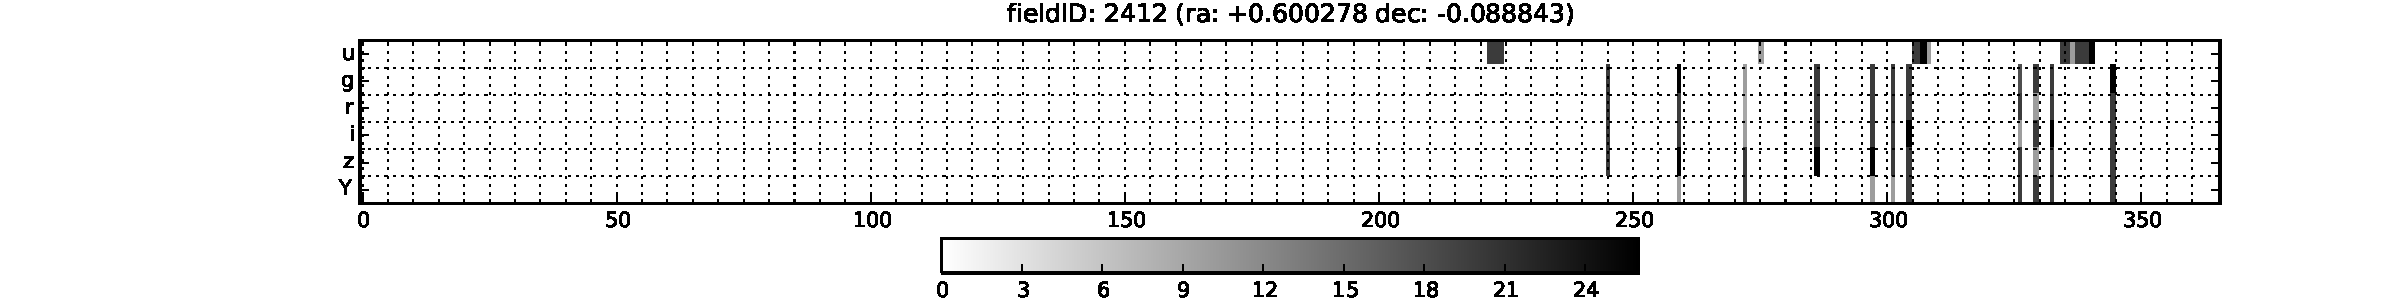
\includegraphics[width=\textwidth]{figs/supernova/fig_firstSeason_3}
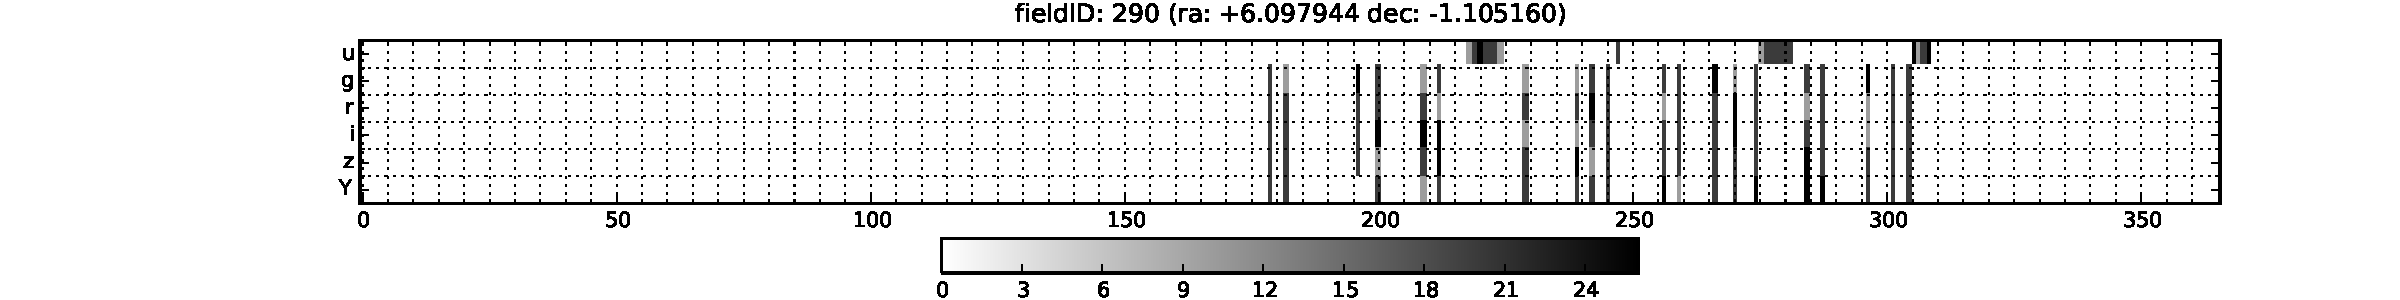
\includegraphics[width=\textwidth]{figs/supernova/fig_firstSeason_4}
\label{fig:opsimSummary}
\caption{Cadence in different filters for a few LSST DDFs in
    the the ouptut of OpSim version Enigma 1189. This ignores issues of chip 
gaps and overlaps between LSST pointings. These issues have been addressed in \citep{CarrollEtal2014} and Awan et.al. (2015, in prep.). We will add these to this analysis.}
\end{figure}



% --------------------------------------------------------------------

\subsection{Discussion}
\label{sec:keyword:discussion}

Discussion: what risks have been identified? What suggestions could be
made to improve this science project's figure of merit, and mitigate
the identified risks?


\begin{itemize}
\item Intrinsic Dispersion, environmental effects, newer analysis methods
\item Follow-up procedures: What is feasible? Where will our training samples for classification and light curve models come from (other experiments, our own 
sub-samples with spectroscopic follow-up?), spectroscopic follow-up of host galaxies. Can hosts be identified?
\item `Systematics': In what ways will the real data not match the assumptions made in analysis. Having a large sample of SN, to understand the astrophysics would be useful for this. 
\end{itemize}


% ====================================================================

\navigationbar


% --------------------------------------------------------------------

% ====================================================================
%+
% NAME:
%    lenstimedelays.tex
%
% ELEVATOR PITCH:
%    Lensed quasars and supernovae provide distance measurements for
%    cosmology. They are a few days to a few weeks in length. To
%    measure them well we need long campaigns (>~3 years) with high
%    night-to-night cadence (better than the standard 5 days if
%    possible, especially as combining all filters might be difficult.)
%
% COMMENTS:
%
%
% BUGS:
%
%
% AUTHORS:
%   Phil Marshall (@drphilmarshall)
%-
% ====================================================================

\section{ Strong Gravitational Lens Time Delays }
\label{sec:lenstimedelays}

\noindent{\it Phil Marshall} % (Writing team)

% This individual section will need to describe the particular
% discoveries and measurements that are being targeted in this section's
% science case. It will be helpful to think of a ``science case" as a
% ``science project" that the authors {\it actually plan to do}. Then,
% the sections can follow the tried and tested format of an observing
% proposal: a brief description of the investigation, with references,
% followed by a technical feasibility piece. This latter part will need
% to be quantified using the MAF framework, via a set of metrics that
% need to be computed for any given observing strategy to quantify its
% impact on the described science case. Ideally, these metrics would be
% combined in a well-motivated figure of merit. The section can conclude
% with a discussion of any risks that have been identified, and how
% these could be mitigated.

A short preamble goes here. What's the context for this science
project? Where does it fit in the big picture?

% --------------------------------------------------------------------

\subsection{Target measurements and discoveries}
\label{sec:lenstimedelays:targets}

Describe the discoveries and measurements you want to make.

Now, describe their response to the observing strategy. Qualitatively,
how will the science project be affected by the observing schedule and
conditions? In broad terms, how would we expect the observing strategy
to be optimized for this science?


% --------------------------------------------------------------------

\subsection{Metrics}
\label{sec:lenstimedelays:metrics}

Quantifying the response via MAF metrics: definition of the metrics,
and any derived overall figure of merit.


% --------------------------------------------------------------------

\subsection{OpSim Analysis}
\label{sec:lenstimedelays:analysis}

OpSim analysis: how good would the default observing strategy be, at
the time of writing for this science project?


% --------------------------------------------------------------------

\subsection{Discussion}
\label{sec:lenstimedelays:discussion}

Discussion: what risks have been identified? What suggestions could be
made to improve this science project's figure of merit, and mitigate
the identified risks?


% ====================================================================


% --------------------------------------------------------------------
